\documentclass[aspectratio=169]{beamer}

%\includeonlyframes{current}

\usepackage[utf8]{inputenc}
\usepackage[american]{babel}
\usepackage{amsmath,amsthm}
\usepackage{unicode}
\usepackage{array,tabularx}
\usepackage{ifthen}
\usepackage{tikz}
\usetikzlibrary{matrix,decorations,decorations.text,calc,arrows,snakes,shapes,positioning}
\usepackage[backend=biber,citestyle=authoryear-comp,bibstyle=beamer,doi=false,isbn=false,url=true,maxnames=10]{biblatex}
\bibliography{refs}

\usepackage{ulem}

\mode<presentation>{%
  \usetheme{ibm}
}

\newcommand{\C}{ℂ}
\newcommand{\R}{ℝ}
\newcommand{\Z}{ℤ}
\newcommand{\N}{ℕ}
\newcommand{\Q}{ℚ}
\newcommand{\F}{\mathbb{F}}
\renewcommand{\P}{\mathbb{P}}
\renewcommand{\O}{\mathcal{O}}
\newcommand{\tildO}{\mathcal{\tilde{O}}}
\newcommand{\poly}{\operatorname{poly}}
\newcommand{\polylog}{\operatorname{polylog}}
\newcommand{\End}{\operatorname{End}}
\newcommand{\Hom}{\operatorname{Hom}}
\newcommand{\Gal}{\operatorname{Gal}}
\newcommand{\chr}{\operatorname{char}}
\newcommand{\Cl}{\operatorname{Cl}}
\newcommand{\GL}{\operatorname{GL}}
\renewcommand{\a}{{\mathfrak{a}}}
\renewcommand{\b}{{\mathfrak{b}}}
\newcommand{\g}{{\mathfrak{g}}}
\newcommand{\G}{{\mathcal{G}}}
\newcommand{\E}{{\mathcal{E}}}
\newcommand{\cyc}[1]{{〈 #1 〉}}
\newcommand{\ord}{\operatorname{ord}}
\newcommand{\mat}[1]{\left(\begin{smallmatrix}#1\end{smallmatrix}\right)}
\newcommand{\from}{\overset{\$}{\leftarrow}}

\newcommand{\bl}[1]{\textcolor{blue}{#1}}
\newcommand{\rd}[1]{\textcolor{red}{#1}}
\newcommand{\gr}[1]{\textcolor{green}{#1}}
\newcommand{\og}[1]{\textcolor{orange}{#1}}

\newcommand{\myedge}[3]{
  \draw[#3] (360/\crater*#1 : \diam) to[bend right] (360/\crater*#2 : \diam);
}
\newcommand{\sk}[4]{
  \draw[very thick,blue]   (0,0) -- (0,#1);
  \draw[very thick,red]    (1,0) -- (1,#2);
  \draw[very thick,green]  (2,0) -- (2,#3);
  \draw[very thick,orange] (3,0) -- (3,#4);
}

\newenvironment<>{goodblock}[1]{%
  \begin{actionenv}#2%
      \def\insertblocktitle{#1}%
      \par%
      \mode<presentation>{%
        \setbeamercolor{block title}{fg=green!60!black,bg=green!50!white}
       \setbeamercolor{block body}{bg=green!20!white}
     }%
      \usebeamertemplate{block begin}}
    {\par\usebeamertemplate{block end}\end{actionenv}}
\newenvironment<>{mehblock}[1]{%
  \begin{actionenv}#2%
      \def\insertblocktitle{#1}%
      \par%
      \mode<presentation>{%
        \setbeamercolor{block title}{fg=yellow!50!black,bg=yellow!50!white}
       \setbeamercolor{block body}{bg=yellow!20!white}
     }%
      \usebeamertemplate{block begin}}
    {\par\usebeamertemplate{block end}\end{actionenv}}
\newenvironment<>{badblock}[1]{%
  \begin{actionenv}#2%
      \def\insertblocktitle{#1}%
      \par%
      \mode<presentation>{%
        \setbeamercolor{block title}{fg=red!60!black,bg=red!50!white}
       \setbeamercolor{block body}{bg=red!20!white}
     }%
      \usebeamertemplate{block begin}}
    {\par\usebeamertemplate{block end}\end{actionenv}}


../share/isographs.tex

\title[Isogeny Based Cryptography]{Isogeny Based Cryptography: an Introduction}
\author{Luca De Feo}
\date[\textcolor{blue}{\url{https://defeo.lu/docet}}~~~~~~Simula UiB]{November 18, 2019\\
  Simula UiB, Bergen\\
  \medskip
  Slides online at \url{https://defeo.lu/docet}}
\institute{IBM Research Zürich}

\begin{document}

\frame[plain]{\titlepage}

%%

\begin{frame}{Why isogenies?}
  \begin{columns}
    \begin{column}{0.45\textwidth}
      Six families still in NIST post-quantum competition:
      
      \bigskip
      \begin{tabular}{ >{\color{structure}}l@{\hspace{2em}} c c}
        Lattices     & 9 encryption & \textcolor{black!30}{3 signature} \\
        Codes        & 7 encryption\\
        Multivariate & & \textcolor{black!30}{4 signature}\\
        Isogenies    & \alert{1 encryption}\\
        Hash-based   & & \textcolor{black!30}{1 signature}\\
        MPC          & & \textcolor{black!30}{1 signature}
      \end{tabular}
    \end{column}
    \begin{column}{0.45\textwidth}<2->
      \centering
      \begin{overlayarea}{0.8\textwidth}{\textheight}
        \begin{onlyenv}<2>
          \begin{tikzpicture}
            \node at (3,-0.5) {\bf Public key size};
            \node at (3,-1) {NIST-1 level (AES128)};
            \node at (3,-1.5) {\footnotesize (not to scale)};
            \draw (0.5,0) -- (5.5,0);
            \fill[structure] (1,0) -- (2,0) -- (2,4) -- (1,4);
            \node at (1.5,4.5) {\parbox{2cm}{\centering \emph{Codes}\\1 -- 300 KB}};
            \fill[structure] (2.5,0) -- (3.5,0) -- (3.5,1) -- (2.5,1);
            \node at (3,1.8) {\parbox{2cm}{\centering \emph{Lattices}\\0.5 -- 10 KB}};
            \fill[structure] (4,0) -- (5,0) -- (5,0.2) -- (4,0.2);
            \node at (4.5,0.7) {\parbox{2cm}{\centering \emph{Isogenies}\\209 B}};
          \end{tikzpicture}
        \end{onlyenv}
        \transdissolve<3>
        \begin{onlyenv}<3->
          \begin{tikzpicture}
            \node at (3,-0.5) {\bf Encryption performance};
            \node at (3,-1) {NIST-1 level (AES128)};
            \node at (3,-1.5) {\footnotesize (not to scale)};
            \draw (0.5,0) -- (5.5,0);
            \fill[structure] (1,0) -- (2,0) -- (2,0.2) -- (1,0.2);
            \node at (1.5,0.7) {\parbox{2cm}{\centering \emph{Codes}\\1 Mcycles}};
            \fill[structure] (2.5,0) -- (3.5,0) -- (3.5,0.3) -- (2.5,0.3);
            \node at (3,1) {\parbox{2cm}{\centering \emph{Lattices}\\0.5 -- 5 Mcycles}};
            \fill[structure] (4,0) -- (5,0) -- (5,4) -- (4,4);
            \node at (4.5,4.5) {\parbox{2cm}{\centering \emph{Isogenies}\\190 Mcycles}};
          \end{tikzpicture}
        \end{onlyenv}
      \end{overlayarea}
    \end{column}
  \end{columns}
\end{frame}

%%

\begin{frame}

  \vfill
  
  \begin{quotation}
    ``We found that CECPQ2 ([NTRU] the ostrich) outperformed CECPQ2b
    ([SIKE] the turkey), for the majority of connections in the
    experiment, indicating that \textbf{fast algorithms with large
      keys may be more suitable for TLS than slow algorithms with
      small keys}. However, \textbf{we observed the opposite}---that
    CECPQ2b outperformed CECPQ2---\textbf{for the slowest connections
      on some devices}, including Windows computers and Android mobile
    devices. One possible explanation for this is packet fragmentation
    and packet loss.''
  \end{quotation}

  \begin{flushright}
    --- K. Kwiatkowski, L. Valenta (Cloudflare)\\
    \emph{The TLS Post-Quantum Experiment}\\
    \small \url{https://blog.cloudflare.com/the-tls-post-quantum-experiment/}
  \end{flushright}
\end{frame}

%% 

\begin{frame}{Weierstrass equations}
  \begin{columns}
    \begin{column}{0.4\textwidth}
      Let $k$ be a field of characteristic $\ne 2,3$.

      An \emph{elliptic curve \textit{defined over $k$}} is the locus
      in $\P^2(\bar{k})$ of an equation
      \[\emph{Y^2Z = X^3 + aXZ^2 + bZ^3},\]
      where $a,b\in k$ and $4a^3+27b^2\ne 0$.

      \begin{itemize}
      \item<2-> $\O=(0:1:0)$ is the \emph{point at infinity};
      \item<3-> $y^2 = x^3 + ax + b$ is the \emph{affine equation}.
      \end{itemize}
    \end{column}
    \begin{column}{0.6\textwidth}
      \begin{center}
        \begin{tikzpicture}[domain=-2.4566:4,samples=100,yscale=1/2]
          \draw plot (\x,{sqrt(\x*\x*\x-4*\x+5)});
          \draw plot (\x,{-sqrt(\x*\x*\x-4*\x+5)});

          \draw[thin,gray,-latex] (0,-7) -- (0,7);
          \draw[thin,gray,-latex] (-3,0) -- (4,0);
        \end{tikzpicture}
      \end{center}
    \end{column}
  \end{columns}
\end{frame}

%%

\begin{frame}{Attention: arithmetic geometry!}
  \begin{columns}
    \begin{column}{0.55\textwidth}
      \[\emph{E \;:\; y^2 = x^3 - 2x + 1}\]

      \bigskip
      
      \emph{Rational} points:
      \begin{itemize}
      \item<1-> $\emph{E(ℚ)} = \{ (1,0), (0,1), (0,-1), \O \}$,
      \item<2-> $\emph{\#E(ℚ(\sqrt{5}))} = 8$,
      \item<3-> \dots
      \item<3-> $\emph{\#E(ℝ)} = ∞$.
      \item<4-> $\emph{\#E(ℂ)} = ∞$.
      \end{itemize}
    \end{column}
    \begin{column}{0.45\textwidth}
      \begin{center}
        \begin{tikzpicture}
          \draw[thin,gray,-latex] (0,-4) -- (0,4);
          \draw[thin,gray,-latex] (-2,0) -- (3,0);

          \draw[fill] (1,0) circle (1pt) (0,1) circle (1pt) (0,-1) circle (1pt);
          \uncover<2->{
            \draw[fill] (-1.61803,0) circle (1pt) (0.61803,0) circle (1pt)
            (2,2.23606) circle (1pt) (2,-2.23606) circle (1pt);
          }

          \begin{uncoverenv}<3->
            \begin{scope}
              [domain=-1.61803:0.61803,samples=50]
              \draw plot (\x,{sqrt(\x*\x*\x-2*\x+1)});
              \draw plot (\x,{-sqrt(\x*\x*\x-2*\x+1)});
            \end{scope}
            \begin{scope}
              [domain=1:2.5,samples=50]
              \draw plot (\x,{sqrt(\x*\x*\x-2*\x+1)});
              \draw plot (\x,{-sqrt(\x*\x*\x-2*\x+1)});
            \end{scope}
          \end{uncoverenv}          
        \end{tikzpicture}
      \end{center}
    \end{column}
  \end{columns}  
\end{frame}

%%

\begin{frame}{The group law}
  \begin{columns}
    \begin{column}{0.4\textwidth}
      \begin{block}{Bezout's theorem}
        Every line cuts $E$ in exactly three points (counted with
        multiplicity).
      \end{block}

      Define a \emph{group law} such that any three colinear points
      add up to zero.

      \begin{itemize}
      \item<2-> The law is \emph{algebraic}\\ (it has \textit{formulas});
      \item<3-> The law is \emph{commutative};
      \item<3-> $\O$ is the \emph{group identity};
      \item<3-> \emph{Opposite points} have the same $x$-value.
      \end{itemize}
    \end{column}
    \begin{column}{0.6\textwidth}
      \begin{center}
        \begin{tikzpicture}[domain=-2.4566:4,samples=100,yscale=1/2]
          \draw plot (\x,{sqrt(\x*\x*\x-4*\x+5)});
          \draw plot (\x,{-sqrt(\x*\x*\x-4*\x+5)});

          \draw[thin,gray,-latex] (0,-7) -- (0,7);
          \draw[thin,gray,-latex] (-3,0) -- (4,0);
          \draw (-3,1) -- (4,8/3+3);
          \begin{scope}[every node/.style={draw,circle,inner sep=1pt,fill},cm={1,2/3,0,0,(0,3)}]
            \node at (-2.287980,0) {};
            \node at (-0.535051,0) {};
            \node at (3.267475,0) {};
          \end{scope}
          \begin{scope}[every node/.style={yshift=0.3cm},cm={1,2/3,0,0,(0,3)}]
            \node at (-2.287980,0) {$P$};
            \node at (-0.535051,0) {$Q$};
            \node at (3.267475,0) {$R$};
          \end{scope}

          \draw[dashed] (3.267475,3.267475*2/3+3) -- (3.267475,-3.267475*2/3-3) 
          node[draw,circle,inner sep=1pt,fill] {}
          node[xshift=-0.1cm,anchor=east] {$P+Q$};
        \end{tikzpicture}
      \end{center}
    \end{column}
  \end{columns}
\end{frame}

%%

\begin{frame}{Maps: isomorphisms}
  \begin{block}{Isomorphisms}
    The only \emph{invertible algebraic maps} between elliptic curves
    are of the form
    \[(x,y) \mapsto (u^2x, u^3y)\]
    for some $u\in\bar{k}$.

    They are \emph{group isomorphisms}.
  \end{block}

  \begin{block}{$j$-Invariant}
    Let $E\;:\;y^2=x^3+ax+b$, its \emph{$j$-invariant} is
    \[j(E) = 1728\frac{4a^3}{4a^3+27b^2}.\]

    Two elliptic curves $E,E'$ are \emph{isomorphic} if and only if
    $j(E)=j(E')$.
  \end{block}
\end{frame}

%%

\begin{frame}{Group structure}
  \begin{block}{Torsion structure}
    Let $E$ be defined over an algebraically closed field $\bar{k}$ of
    characteristic $p$.
    \begin{align*}
      E[m] \simeq\quad& \Z/m\Z\times\Z/m\Z  &\text{if $p\nmid m$,}\\[1em]
                 &\Z/p^e\Z & \text{\emph{ordinary} case,}\\[-1.7em]
      E[p^e] \simeq\Biggl\{& \\[-1.7em]
                 &\{\O\} & \text{\emph{supersingular} case.}
    \end{align*}
  \end{block}

  \vspace{-2mm}
  
  \begin{block}{Finite fields (Hasse's theorem)}
    Let \emph{$E$} be defined over a finite field \emph{$\F_q$}, then
    \[\lvert\#E(\F_q) - q - 1\rvert \le 2\sqrt{q}.\]
    In particular, there exist integers \emph{$n_1$} and
    \emph{$n_2|\gcd(n_1,q-1)$} such that
    \[E(\F_q) ≃ ℤ/n_1ℤ × ℤ/n_2ℤ.\]
  \end{block}
\end{frame}

%%

\begin{frame}
  \frametitle{Maps: what's \alt<2->{\xout{scalar multiplication} an
      isogeny}{scalar multiplication}?}

  \begin{overlayarea}{\textwidth}{4em}
    \Large
    \[
      \alt<3->{\phi}{[n]}
      \;:\; P \mapsto
      \alt<3->{\phi(P)}{\underbrace{P + P + \cdots + P}_{n\text{ times}}}\]
  \end{overlayarea}
  
  \begin{itemize}
  \item A map \emph{$E\to \alt<4->{\xout{E} E'}{E\phantom{\xout{}}}$},
  \item a \emph{group morphism},
  \item with \emph{finite kernel}\\
    \alt<5->{(\xout{the torsion group $E[n]\simeq(ℤ/nℤ)^2$} any
      finite subgroup \emph{$H\subset E$})}{(the torsion group
      \emph{$E[n]\simeq(ℤ/nℤ)^2$})},
  \item \emph{surjective} (in the algebraic closure),
  \item given by \emph{rational maps} of degree \alt<6->{\xout{$n^2$}
      \emph{$\#H$}}{\emph{$n^2$}}.
  \end{itemize}

  \medskip
  
  \begin{uncoverenv}<7->
    (Separable) isogenies $\Leftrightarrow$ finite subgroups:
    \alert{\[0 \to H \to E \overset{\phi}{\to} E' \to 0\]}
  \end{uncoverenv}
\end{frame}

%% 

\begin{frame}{Isogenies: an example over $\F_{11}$}
  \centering
  \begin{tikzpicture}[scale=0.4]
    \begin{scope}
      \node[anchor=center] at (0,7) {$E \;:\; y^2 = x^3 + x$};

      \uncover<-1>{
        \draw[thin,gray] (0,-6) -- (0,6);
        \draw[thin,gray] (-6,0) -- (6,0);
      }

      \foreach \x/\y in {0/0,5/3,-4/3,-3/5,-2/1,-1/3} {
        \draw[blue,fill] (\x,\y) circle (0.2) node(E_\x_\y){}
        (\x,-\y) circle (0.2) node(E_\x_-\y){};
      }

      \uncover<2->{\draw[red,fill] (0,0) circle (0.3);}
    \end{scope}

    \draw[black!10!white,thick] (10,-7) -- +(0,14);
    
    \begin{scope}[shift={(20,0)}]
      \node at (0,7) {$E' \;:\; y^2 = x^3 - 4x$};

      \uncover<-1>{
        \draw[thin,gray] (0,-6) -- (0,6);
        \draw[thin,gray] (-6,0) -- (6,0);
      }

      \foreach \x/\y in {0/0,2/0,3/2,4/2,6/4,-2/0,-1/5} {
        \draw[color=blue,fill] (\x,\y) circle (0.2) node(F_\x_\y){}
        (\x,-\y) circle (0.2) node(F_\x_-\y){};
      }
    \end{scope}

    \begin{scope}[color=red,-latex,dashed]
      \begin{uncoverenv}<2->
        \path
        (E_5_3) edge (F_3_2)
        (E_-4_3) edge (F_4_-2)
        (E_-3_5) edge (F_4_2)
        (E_-2_1) edge (F_3_-2)
        (E_-1_3) edge (F_-2_0);
      \end{uncoverenv}
      \begin{uncoverenv}<2->
        \path
        (E_5_-3) edge (F_3_-2)
        (E_-4_-3) edge (F_4_2)
        (E_-3_-5) edge (F_4_-2)
        (E_-2_-1) edge (F_3_2)
        (E_-1_-3) edge (F_-2_0);
      \end{uncoverenv}
    \end{scope}
  \end{tikzpicture}
  
  \begin{columns}
    \begin{column}{0.5\textwidth}
      \[\phi(x,y) = \left(\frac{x^2 + 1}{x},\quad y\frac{x^2-1}{x^2}\right)\]
    \end{column}
    \begin{column}{0.5\textwidth}
      \begin{itemize}
      \item<2-> Kernel generator in \alert{red}.
      \item<2-> This is a degree $2$ map.
      \item<2-> Analogous to $x\mapsto x^2$ in $\F_q^*$.
      \end{itemize}
    \end{column}
  \end{columns}
\end{frame}

%%

\begin{frame}{Maps: isogenies}
  \begin{theorem}
    Let $\phi:E\to E'$ be a map between elliptic curves. These
    conditions are equivalent:
    \begin{itemize}
    \item $\phi$ is a \emph{surjective group morphism},
    \item $\phi$ is a \emph{group morphism} with \emph{finite kernel},
    \item $\phi$ is a non-constant \emph{algebraic map} of projective
      varieties sending the point at infinity of $E$ onto the point at
      infinity of $E'$.
    \end{itemize}
    If they hold $\phi$ is called an \emph{isogeny}.
  \end{theorem}

  Two curves are called \emph{isogenous} if there exists an isogeny
  between them.

  \begin{block}{Example: Multiplication-by-$m$}
    On any curve, an isogeny from $E$ to itself (i.e., an
    \emph{endomorphism}):
    \begin{align*}
      [m] \;:\; E &\to E,\\
      P &\mapsto [m]P.
    \end{align*}
  \end{block}
\end{frame}

%%

\begin{frame}{Isogeny lexicon}
  \begin{block}{Degree}
    \begin{itemize}
    \item $\approx$ degree of the rational fractions defining the isogeny;
    \item Rough measure of the information needed to encode it.
    \end{itemize}
  \end{block}
  
  \begin{block}{Separable, inseparable, cyclic}
    An isogeny $ϕ$ is \emph{separable} iff \emph{$\degϕ=\#\kerϕ$}.

    \begin{itemize}
    \item Given \emph{$H⊂E$} finite, write \emph{$ϕ : E → E/H$} for
      the \emph{unique} separable isogeny s.t. \emph{$\kerϕ=H$}.
    \item $ϕ$ \emph{inseparable} $⇒$ $p$ divides $\degϕ$.
    \item \emph{Cyclic isogeny} $≡$ separable isogeny with cyclic
      kernel.
      \begin{itemize}
      \item \emph{Non-example:} the multiplication map $[m]:E→E$.
      \end{itemize}
    \end{itemize}
  \end{block}

  \begin{block}{Rationality}
    Given $E$ \emph{defined over $k$}, an isogeny $ϕ$ is rational if
    $\ker ϕ$ is \emph{Galois invariant}.
    \begin{itemize}
    \item[$⇒$] $ϕ$ is represented by rational fractions with
      coefficients in $k$.
    \end{itemize}
  \end{block}
\end{frame}

%%

\begin{frame}{The dual isogeny}
  Let $\phi:E\to E'$ be an isogeny of degree $m$. 
  There is a unique isogeny $\hat{\phi}:E'\to E$ such that
  \[\hat{\phi}\circ\phi = [m]_E, \quad \phi\circ\hat{\phi} = [m]_{E'}.\]
  $\hat{\phi}$ is called the \emph{dual isogeny of $\phi$}; it has the
  following properties:
  
  \begin{enumerate}
  \item $\hat{\phi}$ is defined over $k$ if and only if $\phi$ is;
  \item $\widehat{\psi\circ\phi} = \hat{\phi}\circ\hat{\psi}$ for any isogeny $\psi:E'\to E''$;
  \item $\widehat{\psi+\phi} = \hat{\psi} + \hat{\phi}$ for any isogeny $\psi:E\to E'$;
  \item $\deg \phi = \deg\hat{\phi}$;
  \item $\hat{\hat{\phi}} = \phi$.
  \end{enumerate}
\end{frame}

%%

\begin{frame}{Up to \emph{isomorphism}}
  \begin{center}
    \begin{tikzpicture}[domain=-2.4566:4,samples=100]
      \newcount\zoomout
      \transduration<15-21>{0.5}
      \animatevalue<15-20>{\zoomout}{0}{10}
      \begin{uncoverenv}<-20>
        \begin{scope}[scale=1-0.09*\zoomout]
          \begin{scope}
            \draw[thin,gray,-latex] (0,-4) -- (0,4);
            \draw[thin,gray,-latex] (-4.2,0) -- (7,0);
          \end{scope}
          
          \newcount\xstretch
          \newcount\ystretch
          \newcount\slant
          \transduration<1-13>{0.5}
          \animatevalue<1-5>{\xstretch}{0}{4}
          \animatevalue<5-9>{\ystretch}{0}{4}
          \animatevalue<9-13>{\slant}{0}{4}      
          \begin{scope}[yscale=0.55-0.05*\the\ystretch,xscale=1+0.1*\the\xstretch,xslant=0.02*\slant]
            \draw plot (\x,{sqrt(\x*\x*\x-4*\x+5)});
            \draw plot (\x,{-sqrt(\x*\x*\x-4*\x+5)});

            \begin{uncoverenv}<-18>
              \draw (-3,1) -- (4,8/3+3);
              \begin{scope}[every node/.style={draw,circle,inner sep=1pt,fill},cm={1,2/3,0,0,(0,3)}]
                \node at (-2.287980,0) {};
                \node at (-0.535051,0) {};
                \node at (3.267475,0) {};
              \end{scope}
              \begin{scope}[every node/.style={yshift=0.3cm},cm={1,2/3,0,0,(0,3)}]
                \node at (-2.287980,0) {$P$};
                \node at (-0.535051,0) {$Q$};
                \node at (3.267475,0) {$R$};
              \end{scope}
              \draw[dashed] (3.267475,3.267475*2/3+3) -- (3.267475,-3.267475*2/3-3) 
              node[draw,circle,inner sep=1pt,fill] {}
              node[xshift=-0.1cm,anchor=east] {$P+Q$};
            \end{uncoverenv}
          \end{scope}

          \begin{uncoverenv}<14>
            \node[anchor=west] at (-4,-3) {\Large\alert{$y^2=x^3+ax+b \quad\longrightarrow\quad j\equiv 1728\frac{4a^3}{4a^3+27b^2}$}};
          \end{uncoverenv}
        \end{scope}
      \end{uncoverenv}
      
      \begin{uncoverenv}<21->
        \draw[fill] (0,0) circle (2pt) node[anchor=north] {$j=1728$};
        \uncover<22>{
          \draw (0.1,0) edge[bend left,->] node[auto] {$\phi$} (7,0);
        }
        \uncover<22->{
          \draw[fill] (7.1,0) circle (2pt) node[anchor=north] {$j=287496$};
        }
        \uncover<23->{
          \draw (0.1,0) edge[bend left,<->,red,very thick] (7,0);
        }
      \end{uncoverenv}
    \end{tikzpicture}
  \end{center}  
\end{frame}

%%

\begin{frame}{Isogeny graphs}
  \begin{block}{Serre-Tate theorem}
    Two elliptic curves $E,E'$ defined over a finite field $\F_q$ are
    \emph{isogenous}\\
    (over $\F_q$) iff \emph{$\#E(\F_q) = \#E'(\F_q)$}.
  \end{block}

  \smallskip

  \begin{columns}
    \begin{column}{0.5\textwidth}
      \emph{Isogeny graphs}
      \begin{itemize}
      \item \emph{Vertices are curves} up to isomorphism,
      \item \emph{Edges are isogenies} up to isomorphism.
      \end{itemize}

      \emph{Isogeny volcanoes}
      \begin{itemize}
      \item Curves are ordinary,
      \item Isogenies all have degree a prime $\ell$.
      \end{itemize}
    \end{column}      
    \begin{column}{0.5\textwidth}
      \centering
      \begin{tikzpicture}
        \begin{scope}
          \def\crater{7}
          \foreach \i in {1,...,\crater} {
            \draw[fill] (360/\crater*\i:1cm) circle (5pt);
            \draw (360/\crater*\i : 1cm) -- (360/\crater*\i+360/\crater : 1cm);
            \foreach \j in {-1,1} {
              \draw[fill] (360/\crater*\i : 1cm) -- (360/\crater*\i + \j*360/\crater/4 : 2cm) circle (3pt);
              \foreach \k in {-1,0,1} {
                \draw[fill] (360/\crater*\i + \j*360/\crater/4 : 2cm) --
                (360/\crater*\i + + \j*360/\crater/4 + \k*360/\crater/6 : 2.5cm) circle (1pt);
              }
            }
          }
        \end{scope}
      \end{tikzpicture}
    \end{column}
  \end{columns}
\end{frame}

%%

\begin{frame}{The endomorphism ring}
  The \emph{endomorphism ring} $\End(E)$ of an elliptic curve $E$ is
  the ring of all isogenies $E\to E$ (plus the null map) with
  \emph{addition} and \emph{composition}.

  \begin{block}{Theorem (Deuring)}
    Let $E$ be an elliptic curve defined over a field $k$ of
    characteristic $p$.\\
    $\End(E)$ is isomorphic to one of the following:
    \begin{itemize}
    \item $\Z$, only if $p=0$
      \begin{flushright}
        $E$ is \emph{ordinary}.
      \end{flushright}
    \item An order $\O$ in a quadratic imaginary field:
      \begin{flushright}
        $E$ is \emph{ordinary} with \emph{complex multiplication} by
        $\O$.
      \end{flushright}
    \item Only if $p>0$, a maximal order in a quaternion
      algebra\footnote{(ramified at $p$ and $\infty$)}:
      \begin{flushright}
        $E$ is \emph{supersingular}.
      \end{flushright}
    \end{itemize}
  \end{block}
\end{frame}

%%

\begin{frame}{Algebras, orders}
  \begin{itemize}
  \item A \emph{quadratic imaginary number field} is an extension of
    $\Q$ of the form $\Q(\sqrt{-D})$ for some non-square $D>0$.
  \item A \emph{quaternion algebra} is an algebra of the form
    $\Q + \alpha\Q + \beta\Q + \alpha\beta\Q$, where the generators
    satisfy the relations
    \[\alpha^2,\beta^2\in\Q, \quad \alpha^2<0, \quad \beta^2 < 0, \quad \beta\alpha=-\alpha\beta.\]
  \end{itemize}
  
  \begin{block}{Orders}
    Let $K$ be a finitely generated $\Q$-algebra.  An \emph{order}
    $\O\subset K$ is a \emph{subring} of $K$ that is a finitely
    generated $\Z$-module of \emph{maximal dimension}.  An order that
    is not contained in any other order of $K$ is called a
    \emph{maximal order}.
  \end{block}

  \begin{description}
  \item[Examples:]
    \begin{itemize}
    \item $\Z$ is the only order contained in $\Q$,
    \item $\Z[i]$ is the only maximal order of $\Q(i)$,
    \item $\Z[\sqrt{5}]$ is a non-maximal order of $\Q(\sqrt{5})$,
    \item The \emph{ring of integers} of a number field is its only
      maximal order,
    \item In general, maximal orders in quaternion algebras are
      \emph{not unique}.
    \end{itemize}
  \end{description}
\end{frame}

%%

\begin{frame}{The finite field case}
  \begin{block}{Theorem (Hasse)}
    Let $E$ be defined over a finite field. Its Frobenius endomorphism
    $\pi$ satisfies a quadratic equation
    \[\pi^2 - t\pi + q = 0\]
    in $\End(E)$ for some $|t|\le2\sqrt{q}$, called the \emph{trace}
    of $\pi$.  The trace $t$ is coprime to $q$ if and only if $E$ is
    ordinary.
  \end{block}

  Suppose $E$ is \emph{ordinary}, then $D_\pi=t^2-4q<0$ is the
  \emph{discriminant} of $\Z[\pi]$.
  
  \begin{itemize}
  \item $K=\Q(\pi)=\Q(\sqrt{D_\pi})$ is the \emph{endomorphism algebra} of $E$.
  \item Denote by $\O_K$ its ring of integers, then
    \[\Z \ne \Z[\pi] \subset \End(E) \subset \O_K.\]
  \end{itemize}

  In the \emph{supersingular} case, $\pi$ may or may not be in $\Z$,
  depending on $q$.
\end{frame}

%%

\begin{frame}{Endomorphism rings of ordinary curves}
  \begin{columns}
    \begin{column}{0.55\textwidth}
      \begin{block}{Classifying quadratic orders}
        Let $K$ be a quadratic number field, and let $\O_K$ be its ring of
        integers.
        \begin{itemize}
        \item Any order $\O\subset K$ can be written as $\O=\Z+f\O_K$ for
          an integer $f$, called the \emph{conductor} of $\O$, denoted by
          $[\O_K:\O]$.
        \item If $d_K$ is the \emph{discriminant} of $K$, the discriminant
          of $\O$ is $f^2d_K$.
        \item If $\O,\O'$ are two orders with discriminants $d,d'$, then
          \emph{$\O\subset\O'$ iff $d'|d$}.
        \end{itemize}
      \end{block}
    \end{column}
    \begin{column}{0.4\textwidth}
      \centering
      \begin{tikzpicture}[xscale=2.2,yscale=2]
        \node(OK) at (0,0) {$\O_K$};
        \node(O2) at (-1,-1) {$\Z+2\O_K$};
        \node(O3) at (0,-1) {$\Z+3\O_K$};
        \node(O5) at (1,-1) {$\Z+5\O_K$};
        \node(O6) at (-1,-2) {$\Z+6\O_K$};
        \node(O10) at (0,-2) {$\Z+10\O_K$};
        \node(O15) at (1,-2) {$\Z+15\O_K$};
        \node(O30) at (0,-3) {$\Z[\pi]\simeq\Z+30\O_K$};

        \begin{scope}
          \draw
          (OK) edge (O2) edge (O3) edge (O5)
          (O2) edge (O6) edge (O10)
          (O3) edge (O6) edge (O15)
          (O5) edge (O10) edge (O15)
          (O30) edge (O6) edge (O15) edge (O10);
        \end{scope}
      \end{tikzpicture}
    \end{column}
  \end{columns}
\end{frame}

%%

\begin{frame}{Volcanology (Kohel 1996)}

  \begin{columns}
    \begin{column}{0.4\textwidth}
      Let \emph{$E,E'$} be curves with respective endomorphism rings \emph{$\O,\O'⊂K$}.\\
      Let \emph{$ϕ:E→E'$} be an isogeny of prime degree \emph{$ℓ$},
      then:

      \bigskip
      
      \begin{tabular}{l l}
        if $\O=\O'$, & $ϕ$ is \emph{horizontal};\\
        if $[\O':\O]=ℓ$, & $ϕ$ is \emph{ascending};\\
        if $[\O:\O']=ℓ$, & $ϕ$ is \emph{descending}.
      \end{tabular}      
    \end{column}
    \begin{column}{0.55\textwidth}
      \centering
      \begin{tikzpicture}
        \def\crater{7}
        \foreach \i in {1,...,\crater} {
          \draw[fill] (360/\crater*\i:1cm) circle (5pt);
          \draw (360/\crater*\i : 1cm) -- (360/\crater*\i+360/\crater : 1cm);
          \foreach \j in {-1,1} {
            \draw[fill] (360/\crater*\i : 1cm) -- (360/\crater*\i + \j*360/\crater/4 : 2cm) circle (3pt);
            \foreach \k in {-1,0,1} {
              \draw[fill] (360/\crater*\i + \j*360/\crater/4 : 2cm) --
              (360/\crater*\i + + \j*360/\crater/4 + \k*360/\crater/6 : 2.5cm) circle (1pt);
            }
          }
        }
        \begin{scope}[xshift=4cm]
          \node at (0,2) {$\End(E)$};
          \draw[fill] (0,1) circle(5pt) node[xshift=0.7cm]{$\O_K$} -- 
          (0,0) circle(3pt) --
          (0,-1) circle(1pt) node[xshift=0.7cm]{$ℤ[π]$};
        \end{scope}
      \end{tikzpicture}
      
      \small
      Ordinary isogeny volcano of degree $ℓ=3$.
    \end{column}
  \end{columns}
\end{frame}

%%

\begin{frame}{Volcanology (Kohel 1996)}
  \centering
  \begin{columns}
    \begin{column}{0.35\textwidth}
      Let $E$ be ordinary, \emph{$\End(E)⊂K$}.

      \bigskip

      $\O_K$: \emph{maximal order} of $K$,\\
      $D_K$: \emph{discriminant} of $K$.

      \bigskip
      
      \uncover<2->{Height \emph{$= v_ℓ([\O_K:ℤ[π]])$}.}
      
      \bigskip
      
      \uncover<3->{\alert{How large is the crater?}}
    \end{column}
    \begin{column}{0.65\textwidth}
      \centering
      \begin{tikzpicture}[scale=0.8]
        \small
        \begin{scope}
          \draw[fill] (0,0) circle (2pt)
          -- (-1,-1) circle (2pt)
          (0,0) -- (0,-1) circle (2pt)
          (0,0) -- (1,-1) circle (2pt);
          \node at (0,-2) {$\left(\frac{D_K}{ℓ}\right) = -1$};
        \end{scope}    

        \begin{scope}[xshift=3.5cm]
          \draw[fill] (0,0) circle (2pt)
          -- (-0.5,-1) circle (2pt)
          (0,0) -- (0.5,-1) circle (2pt)
          (0,0) -- (2,0) circle (2pt)
          -- (1.5,-1) circle (2pt)
          (2,0) -- (2.5,-1) circle (2pt);
          \node at (1,-2) {$\left(\frac{D_K}{ℓ}\right) = 0$};
        \end{scope}
        
        \begin{scope}[xshift=2.5cm,yshift=-3cm]
          \draw[fill] (-0.8,0) node[coordinate] (A) {} circle (2pt)
          -- +(0,-1) circle (2pt)
          (0,-0.3) node[coordinate] (B) {} circle (2pt)
          -- +(0,-1) circle (2pt)
          (0.8,0) node[coordinate] (C) {} circle (2pt)
          -- +(0,-1) circle (2pt);
          \draw[bend right=20]
          (A) edge (B)
          (B) edge (C)
          (C) edge[dashed,bend right=90] (A);
          \node at (0,-2) {$\left(\frac{D_K}{ℓ}\right) = +1$};
        \end{scope}
      \end{tikzpicture}
    \end{column}  
  \end{columns}
  
  \bigskip
  
  \begin{tabular}{c | c | c c c}
    && \textbf{Horizontal} & \textbf{Ascending} & \textbf{Descending}\\
    \hline
    $\ell\nmid[\O_K:\O]$ & $\ell\nmid[\O:ℤ[π]]$ &$1+\left(\frac{D_K}{ℓ}\right)$& &\\
    $\ell\nmid[\O_K:\O]$ & $\ell\mid[\O:ℤ[π]]$ &$1+\left(\frac{D_K}{ℓ}\right)$& &$\ell-\left(\frac{D_K}{ℓ}\right)$\\
    $\ell\mid[\O_K:\O]$ & $\ell\mid[\O:ℤ[π]]$ &  &$1$&$\ell$\\
    $\ell\mid[\O_K:\O]$ & $\ell\nmid[\O:ℤ[π]]$ & &$1$& 
  \end{tabular}
\end{frame}

%%

\begin{frame}{How large is the crater of a volcano?}
  
  Let \emph{$\End(E) = \O \subset ℚ(\sqrt{-D})$}. Define

  \begin{itemize}
  \item $\mathcal{I}(\O)$, the group of \emph{invertible fractional ideals},
  \item $\mathcal{P}(\O)$, the group of \emph{principal ideals},
  \end{itemize}
  
  \begin{block}{The class group}
    The \emph{class group} of $\O$ is
    \[\Cl(\O) = \mathcal{I}(\O)/\mathcal{P}(O).\]
  \end{block}

  \begin{itemize}
  \item It is a \emph{finite abelian} group.
  \item Its order \emph{$h(\O)$} is called the \emph{class number} of
    $\O$.
  \item It arises as the Galois group of an abelian extension of
    $ℚ(\sqrt{-D})$.
  \end{itemize}
\end{frame}

%%

\begin{frame}
  \frametitle{Complex multiplication}

  \begin{block}{The $\a$-torsion}
    Let \emph{$\a\subset\O$} be an (integral invertible) ideal of
    $\O$; Let \emph{$E[\a]$} be the subgroup of $E$ annihilated by
    $\a$:
    \[E[\a] = \{P\in E \;|\; \alpha(P) = 0 \text{ for all }
      \alpha\in\a\};\] %
    Let \emph{$\phi:E\to E_\a$}, where $E_\a=E/E[\a]$.  Then
    $\End(E_\a) = \O$ (i.e., $\phi$ is \emph{horizontal}).
  \end{block}
  \begin{theorem}[Complex multiplication]
    The action on the set of elliptic curves with complex
    multiplication by $\O$ defined by \emph{$\a\ast j(E) = j(E_\a)$}
    factors through $\Cl(\O)$, is faithful and transitive.
  \end{theorem}

  \begin{corollary}
    Let $\End(E)$ have discriminant $D$. Assume that
    $\left(\frac{D}{\ell}\right)=1$, then $E$ is on a crater \emph{of
      size $N$} of an $\ell$-volcano, and \emph{$N|h(\End(E))$}.
  \end{corollary}
\end{frame}

%%

\begin{frame}
  \frametitle{Complex multiplication graphs}
  \begin{center}
    \begin{tikzpicture}
      \begin{scope}
        \def\crater{12}
        \def\jumpa{-8}
        \def\jumpb{9}
        \def\diam{3cm}

        \foreach \i in {1,...,\crater} {
          \uncover<2->{\draw[blue] (360/\crater*\i : \diam) to[bend right] (360/\crater*\i+360/\crater : \diam);}
          \uncover<3->{\draw[red] (360/\crater*\i : \diam) to[bend right] (360/\crater*\i+\jumpa*360/\crater : \diam);}
          \uncover<4->{\draw[green] (360/\crater*\i : \diam) to[bend right=50] (360/\crater*\i+\jumpb*360/\crater : \diam);}
        }
        \foreach \i in {1,...,\crater} {
          \draw[fill] (360/\crater*\i: \diam) circle (2pt) +(360/\crater*\i: 0.4) node{$E_{\i}$};
        }
      \end{scope}
      \begin{scope}[xshift=4.2cm]
        \draw (0,2) node[anchor=west] {\parbox{6cm}{%
            Vertices are elliptic curves \emph{with complex
              multiplication by $\O_K$} (i.e., $\End(E)\simeq\O_K\subset ℚ(\sqrt{-D})$).\\
            \uncover<2->{Edges are \emph{horizontal isogenies} of
              bounded prime degree.}  }};
      
        \uncover<2->{\draw[blue] (0,0) -- (0.5,0)
          (0.5,0) node[anchor=west] {degree $2$};}
        \uncover<3->{\draw[red] (0,-1) -- (0.5,-1) (0.5,-1)
          node[anchor=west] {degree $3$};}
        \uncover<4->{\draw[green]
          (0,-2) -- (0.5,-2) (0.5,-2) node[anchor=west] {degree $5$};}

        \uncover<5->{\draw (0,-3) node[anchor=west] {\parbox{6cm}{%
              Isomorphic to a \emph{Cayley graph of $\Cl(\O_K)$}.}};}
      \end{scope}
    \end{tikzpicture}
  \end{center}
\end{frame}

%%

\begin{frame}{Supersingular endomorphisms}
  Recall, a curve $E$ over a field $\F_q$ of characteristic $p$ is
  \emph{supersingular} iff
  \[π^2 - tπ + q = 0\]
  with \emph{$t=0\mod p$}.

  \begin{block}{Case: $\quad t=0 \quad⇒\quad D_π = -4q$}
    \begin{itemize}
    \item Only possibility for $E/\F_p$,
    \item $E/\F_p$ has \emph{CM by an order of $ℚ(\sqrt{-p})$}, similar
      to the ordinary case.
    \end{itemize}
  \end{block}

  \begin{block}{Case: $\quad t=±2\sqrt{q} \quad⇒\quad D_π = 0$}
    \begin{itemize}
    \item General case for $E/\F_{q}$, when $q$ is an even power.
    \item $π = ±\sqrt{q} \in \Z$, hence \emph{no complex multiplication}.
    \end{itemize}
  \end{block}

  We will ignore marginal cases: $t=±\sqrt{q},±\sqrt{2q},±\sqrt{3q}$.
\end{frame}

%%

\begin{frame}{Supersingular complex multiplication}
  Let \emph{$E/\F_p$} be a \emph{supersingular} curve, then
  \emph{$π^2 = -p$}.

  \begin{block}{Theorem (Delfs, Galbraith 2016)}
    Let \emph{$\End_{\F_p}(E)$} denote the ring of
    \emph{$\F_p$-rational} endomorphisms of $E$.
    Then
    \[ℤ[π] ⊂ \End_{\F_p}(E) ⊂ ℚ(\sqrt{-p}).\]
  \end{block}
  
  \begin{block}{Orders of $ℚ(\sqrt{-p})$}
    \begin{itemize}
    \item If $p=1 \bmod 4$, then \emph{$ℤ[π]$} is the maximal order.
    \item If $p=-1 \bmod 4$, then \emph{$ℤ[\frac{π+1}{2}]$} is the
      maximal order,
      and \emph{$[ℤ[\frac{π+1}{2}]:ℤ[π]]=2$}.
    \end{itemize}
  \end{block}
\end{frame}  

%%

\begin{frame}{Supersingular CM graphs}
  
  \begin{block}{$2$-volcanoes, $p=-1 \bmod 4$}
    \centering
    \begin{tikzpicture}[scale=0.8]
      \def\crater{7}
      \begin{scope}
        \foreach \i in {1,...,\crater} {
          \draw[fill] (360/\crater*\i:1cm) circle (3pt);
          \draw (360/\crater*\i : 1cm) -- (360/\crater*\i+360/\crater : 1cm);
          \draw[fill] (360/\crater*\i : 1cm) -- (360/\crater*\i : 1.5cm) circle (1pt);
        }
      \end{scope}
      \begin{scope}[xshift=4cm]
        \foreach \i in {1,...,\crater} {
          \draw[fill] (360/\crater*\i:1cm) circle (3pt);
          \foreach \j in {-1,0,1} {
            \draw[fill] (360/\crater*\i : 1cm) -- (360/\crater*\i + \j*360/\crater/4 : 1.5cm) circle (1pt);
          }
        }
      \end{scope}
      \begin{scope}[xshift=8cm]
        \draw[fill] (0,0.7) circle(3pt) node[anchor=west,xshift=0.1cm]{$ℤ[\frac{π+1}{2}]$} -- 
        (0,-0.7) circle(1pt) node[anchor=west,xshift=0.1cm]{$ℤ[π]$};
      \end{scope}
    \end{tikzpicture}
  \end{block}

  \begin{block}{$2$-graphs, $p=1\bmod 4$}
    \centering
    \begin{tikzpicture}[scale=0.8]
      \begin{scope}
        \def\crater{10}
        \foreach \i in {1,...,\crater/2} {
          \draw[fill] (360/\crater*2*\i:1cm) circle (2pt);
          \draw[fill] (360/\crater*2*\i : 1cm) -- (360/\crater*2*\i+360/\crater : 1cm) circle (2pt);
        }
      \end{scope}
      \begin{scope}[xshift=6cm]
        \draw[fill] (0,0) circle(2pt) node[anchor=west,xshift=0.1cm]{$ℤ[π]$};
      \end{scope}
    \end{tikzpicture}    
  \end{block}

  \begin{center}
    All \emph{other $ℓ$-graphs are cycles} of horizontal isogenies iff
    $\left(\frac{-p}{ℓ}\right)=1$.
  \end{center}
\end{frame}

%%

\begin{frame}{The full endomorphism ring}
  \begin{block}{Theorem (Deuring)}
    Let $E$ be a \emph{supersingular} elliptic curve, then
    \begin{itemize}
    \item $E$ is isomorphic to a curve defined over \emph{$\F_{p^2}$};
    \item Every \emph{isogeny} of $E$ is defined over \emph{$\F_{p^2}$};
    \item Every \emph{endomorphism} of $E$ is defined over
      \emph{$\F_{p^2}$};
    \item $\End(E)$ is isomorphic to a \emph{maximal order} in a
      \emph{quaternion algebra} ramified at $p$ and $∞$.
    \end{itemize}
  \end{block}

  In particular:
  \begin{itemize}
  \item If $E$ is defined over $\F_p$, then \emph{$\End_{\F_p}(E)$ is
      strictly contained in $\End(E)$}.
  \item Some endomorphisms \emph{do not commute}!
  \end{itemize}
\end{frame}

%%

\begin{frame}{An example}
  The curve of $j$-invariant \emph{$1728$}
  \[E: y^2 = x^3 + x\]
  is supersingular over $\F_p$ iff $p=-1\mod 4$.

  \begin{block}{Endomorphisms}
    \emph{$\End(E) = ℤ〈ι,π〉$}, with:
    \begin{itemize}
    \item $π$ the Frobenius endomorphism, s.t. \emph{$π^2=-p$};
    \item $ι$ the map
      \[ι(x,y) = (-x,iy),\]
      where \emph{$i∈\F_{p^2}$} is a 4-th root of unity.
      Clearly, \emph{$ι^2=-1$}.
    \end{itemize}
    And \emph{$ιπ=-πι$}.
  \end{block}
\end{frame}

%%

\begin{frame}{Class group action party}
  \centering
  \begin{tikzpicture}[scale=2]
    \def\crater{11}
    \draw[fill] (360/\crater:1cm) circle (1pt);
    \uncover<1-2>{
      \draw (360/\crater:1.1cm) node[anchor=west] {$j=1728$};
    }
    \uncover<2->{
      \foreach \i in {1,...,\crater} {
        \draw[fill] (360/\crater*\i:1cm) circle (1pt);
        \draw (360/\crater*\i : 1cm) -- (360/\crater*\i+360/\crater : 1cm);
      }
      \draw (0,0) node {$\Cl(-4p)$};
    }
    \uncover<3->{
      \draw (360/\crater:1.5cm) circle (0.5cm) node {$\Cl(-4)$};
    }
    \uncover<4>{
      \draw (360/\crater*4:1.2cm) node[anchor=south east] {$j=0$};
    }
    \uncover<5->{
      \draw (360/\crater*4:1.5cm) circle (0.5cm) node {$\Cl(-3)$};
    }
    \uncover<6->{
      \begin{scope}[shift={(360/\crater*6:1.7cm)}]
        \foreach \i in {0,...,2} {
          \draw[fill] (360/\crater*6 - 120*\i - 180 : 0.7cm) circle (1pt);
          \draw (360/\crater*6 - 120*\i - 180 : 0.7cm) -- (360/\crater*6 - 120*\i+120 - 180 : 0.7cm);
        }
        \draw (0,0) node {$\Cl(-23)$};
      \end{scope}
      \begin{scope}[shift={(360/\crater*10:1.5cm)}]
        \foreach \i in {0,...,4} {
          \draw[fill] (360/\crater*10 - 72*\i - 180 : 0.5cm) circle (1pt);
          \draw (360/\crater*10 - 72*\i - 180 : 0.5cm) -- (360/\crater*10 - 72*\i+72 - 180 : 0.5cm);
        }
        \draw (0,0) node {$\Cl(-79)$};
      \end{scope}
    }
  \end{tikzpicture}
\end{frame}

%%

\begin{frame}{Supersingular graphs}
  \begin{columns}
    \begin{column}{0.6\textwidth}
      \begin{itemize}
      \item Quaternion algebras have \emph{many maximal orders}.
      \item For every \emph{maximal order type} of $B_{p,\infty}$
        there are \emph{$1$ or $2$ curves over $\F_{p^2}$} having
        endomorphism ring isomorphic to it.
      \item There is a \emph{unique isogeny class} of supersingular
        curves over $\bar{\F}_p$ of size \emph{$≈ p/12$}.
      \item Left ideals act on the set of maximal orders like isogenies.
      \item The graph of \emph{$\ell$}-isogenies is
        \emph{$(\ell+1)$}-regular.
      \end{itemize}
    \end{column}
    \begin{column}{0.4\textwidth}
      \centering
      \begin{tikzpicture}
        \begin{scope}[every node/.style={fill,black,circle,inner sep=2pt}]
          \node at (0,0)  (1){};
          \node at (0,4) (20){};
          \node at (2,1)  (16z){};
          \node at (-2,1)  (81z){};
          \node at (-1,2) (77z){};
          \node at (1,2)  (20z){};
          \node at (-2,3)  (85z){};
          \node at (2,3)  (12z){};
        \end{scope}

        \begin{scope}[red]
          \path (1) edge (85z) edge (81z) edge (12z) edge (16z);
          \path (20) edge (85z) edge (77z) edge (20z) edge (12z);
          \path (81z) edge (85z) edge (77z) edge (16z);
          \path (85z) edge (12z);
          \path (12z) edge (16z);
          \path (16z) edge (20z);
          \path (20z) edge[bend right=10] (77z) edge[bend left=10] (77z);
        \end{scope}
      \end{tikzpicture}
      
      \small
      \emph{Figure:} $3$-isogeny graph on $\F_{97^2}$.
    \end{column}
  \end{columns}
\end{frame}

%%

\begin{frame}{Graphs lexicon}
  \begin{description}
  \item[Degree:] Number of (outgoing/ingoing) edges.
  \item[$k$-regular:] All vertices have degree $k$.
  \item[Connected:] There is a path between any two vertices.
  \item[Distance:] The length of the shortest path between two vertices.
  \item[Diameter:] The longest distance between two vertices.
  \item[$\lambda_1\ge\cdots\ge\lambda_n$:] The (ordered) eigenvalues
    of the adjacency matrix.
  \end{description}
\end{frame}

%%

\begin{frame}{Expander graphs}
  \begin{block}{Proposition}
    If $G$ is a $k$-regular graph, its largest and smallest
    eigenvalues satisfy
    \[k = \lambda_1 \ge \lambda_n \ge -k.\]
  \end{block}
  
  \begin{block}{Expander families}
    An infinite family of connected $k$-regular graphs on $n$ vertices
    is an \emph{expander family} if there exists an $\epsilon>0$ such
    that all \emph{non-trivial} eigenvalues satisfy
    $|\lambda| \le (1-\epsilon)k$ for $n$ large enough.
  \end{block}
  
  \begin{itemize}
  \item Expander graphs have \emph{short diameter}: $O(\log n)$;
  \item Random walks \emph{mix rapidly}: after $O(\log n)$ steps,
    the induced distribution on the vertices is close to uniform.
  \end{itemize}
\end{frame}

%%

\begin{frame}{Expander graphs from isogenies}
  \begin{block}{Theorem (Pizer)}
    Let $\ell$ be fixed. The family of graphs of \emph{supersingular}
    curves over $\F_{p^2}$ with $\ell$-isogenies, as $p\to\infty$, is
    an expander family\footnote{Even better, it has the Ramanujan
      property.}.
  \end{block}
  
  \begin{block}{Theorem (Jao, Miller, Venkatesan)}
    Let $\O\subset\Q(\sqrt{-D})$ be an order in a quadratic imaginary
    field. The graphs of all curves over $\F_q$ with \emph{complex
      multiplication by $\O$}, with isogenies of prime degree
    bounded\footnote{May contain traces of GRH.} by
    $(\log q)^{2+\delta}$, are expanders.
  \end{block}
\end{frame}

%%

\begin{frame}{Executive summary}
  \begin{itemize}
  \item Separable $ℓ$-isogeny = finite kernel = subgroup of $E[ℓ]$ (=
    ideal of norm $\ell$),
  \item Isogeny graphs have $j$-invariants for vertices and ``some''
    isogenies for edges.
  \item By varying the choices for the vertex and the isogeny set, we
    obtain graphs with different properties.
  \item $ℓ$-isogeny graphs of ordinary curves are volcanoes, (full)
    $ℓ$-isogeny graphs of supersingular curves are finite
    $(ℓ+1)$-regular.
  \item CM theory naturally leads to define graphs of horizontal
    isogenies (both in the ordinary and the supersingular case) that
    are isomorphic to Cayley graphs of class groups.
  \item CM graphs are expanders. Supersingular full $ℓ$-isogeny graphs
    are Ramanujan.
  \end{itemize}
\end{frame}

%%

\frame[plain]{\titlepage}

%%

\begin{frame}{The beauty and the beast {\quad\footnotesize(credit: Lorenz Panny)}}
  \begin{overlayarea}{\textwidth}{\textheight}
    \smallskip
    \begin{center}

      \only<-2>{
        Components of particular isogeny graphs look like this:
      }
      \only<3->{
        At this time, there are \underline{\smash{two distinct families}} of systems:
      }
      \par\vspace{1ex}

      \begin{minipage}{.49\textwidth}\centering
        \begin{tikzpicture}[scale=.6,>=stealth,shorten >=.2mm,shorten <=.2mm,rotate=90,line width=.6pt]
          \isoggraph
        \end{tikzpicture}

        \vspace{.2ex}

        \only<3->{
          $\F_p$ \\[.7ex]
          \textbf{CSIDH}
          \,\raisebox{.2ex}{\small{[pron.: sea-side]}}
          \\ {\small
            \url{https://csidh.isogeny.org}
            \par}
        }
      \end{minipage}
      % 
      \begin{minipage}{.49\textwidth}\centering
        \begin{tikzpicture}[scale=2.456,>=stealth,shorten >=.2mm,shorten <=.2mm,rotate=90,line width=.6pt]
          \fpsqgraph
        \end{tikzpicture}

        \vspace{.2ex}

        \only<3->{
          $\F_{p^2}$ \\[.7ex]
          \textbf{SIDH}
          \\ {\small
            \url{https://sike.org}
            \par}
        }
      \end{minipage}

      \only<-2>{
        \vspace{3ex}

        \textit{Which of these is good for crypto?}
        \pause
        \onslide<2>{%
          \,\textbf{Both.}
        }
      }

    \end{center}
  \end{overlayarea}
\end{frame}

%%

\begin{frame}{Brief history of isogeny-based cryptography}
  \begin{description}
  \item[1997] Couveignes introduces the \emph{Hard Homogeneous Spaces}
    framework. His work stays unpublished for 10 years.
  \item[2006] Rostovtsev \& Stolbunov independently rediscover
    Couveignes ideas, suggest isogeny-based Diffie--Hellman as a
    \emph{quantum-resistant} primitive.
  \item[2006-2010] Other isogeny-based protocols by Teske and Charles,
    Goren \& Lauter.
  \item[2011-2012] D., Jao \& Plût introduce \emph{SIDH}, an
    efficient post-quantum key exchange inspired by Couveignes,
    Rostovtsev, Stolbunov, Charles, Goren, Lauter.
  \item[2017] SIDH is submitted to the NIST competition (with the name
    \emph{SIKE}, only isogeny-based candidate).
  \item[2018] D., Kieffer \& Smith \textit{resurrect} the
    Couveignes--Rostovtsev--Stolbunov protocol, Castryck, Lange,
    Martindale, Panny \& Renes create an efficient variant named
    \emph{CSIDH}.
  \item[2019] The year of proofs of isogeny knowledge: \emph{SeaSign}
    (D. \& Galbraith; Decru, Panny \& Vercauteren), \emph{CSI-FiSh}
    (Beullens, Kleinjung \& Vercauteren), \emph{VDF} (D., Masson,
    Petit \& Sanso), \emph{threshold} (D. \& Meyer).
  \end{description}
\end{frame}

%%

\begin{frame}{Elliptic curves}

  Let \emph{$E \;:\; y^2 = x^3 + ax + b$} be an elliptic curve\dots

  \begin{center}
    \begin{tikzpicture}[domain=-2.4566:4,samples=100]
      \newcount\rotate
      \animate<2-6>
      \animatevalue<2-6>{\rotate}{0}{90}
      \begin{scope}[rotate=-\the\rotate]
        \draw plot (\x,{0.5*sqrt(\x*\x*\x-4*\x+5)});
        \draw plot (\x,{-0.5*sqrt(\x*\x*\x-4*\x+5)});
      \end{scope}
      
      \begin{uncoverenv}<1>
        \begin{scope}[yscale=1/2]
          \draw[thin,gray,-latex] (0,-7) -- (0,7);
          \draw[thin,gray,-latex] (-3,0) -- (4,0);
          
          \draw (-3,1) -- (4,8/3+3);
          \begin{scope}[every node/.style={draw,circle,inner sep=1pt,fill},cm={1,2/3,0,0,(0,3)}]
            \node at (-2.287980,0) {};
            \node at (-0.535051,0) {};
            \node at (3.267475,0) {};
          \end{scope}
          \begin{scope}[every node/.style={yshift=0.3cm},cm={1,2/3,0,0,(0,3)}]
            \node at (-2.287980,0) {$P$};
            \node at (-0.535051,0) {$Q$};
            \node at (3.267475,0) {$R$};
          \end{scope}
          \draw[dashed] (3.267475,3.267475*2/3+3) -- (3.267475,-3.267475*2/3-3) 
          node[draw,circle,inner sep=1pt,fill] {}
          node[xshift=-0.1cm,anchor=east] {$P+Q$};
        \end{scope}
      \end{uncoverenv}
    \end{tikzpicture}
  \end{center}
\end{frame}

%%

\begin{frame}{Elliptic curves}
  \transdissolve
  \centering
  
\includegraphics[height=0.7\textheight]{ec-happy}
\end{frame}

%%

\begin{frame}{The QUANTHOM Menace}
  \centering
  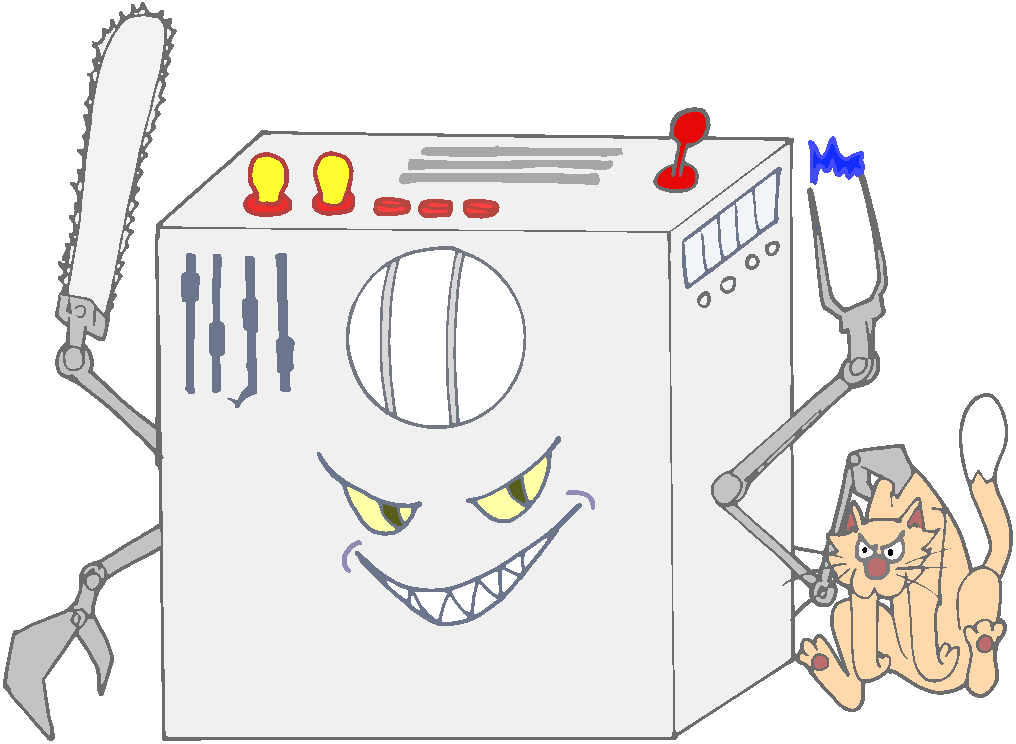
\includegraphics[height=0.7\textheight]{qc-color}
\end{frame}

%%

\begin{frame}{Basically every isogeny-based key-exchange...}
  \centering
  \begin{tikzpicture}
    \comicneue\itshape
    \node at (0,0) {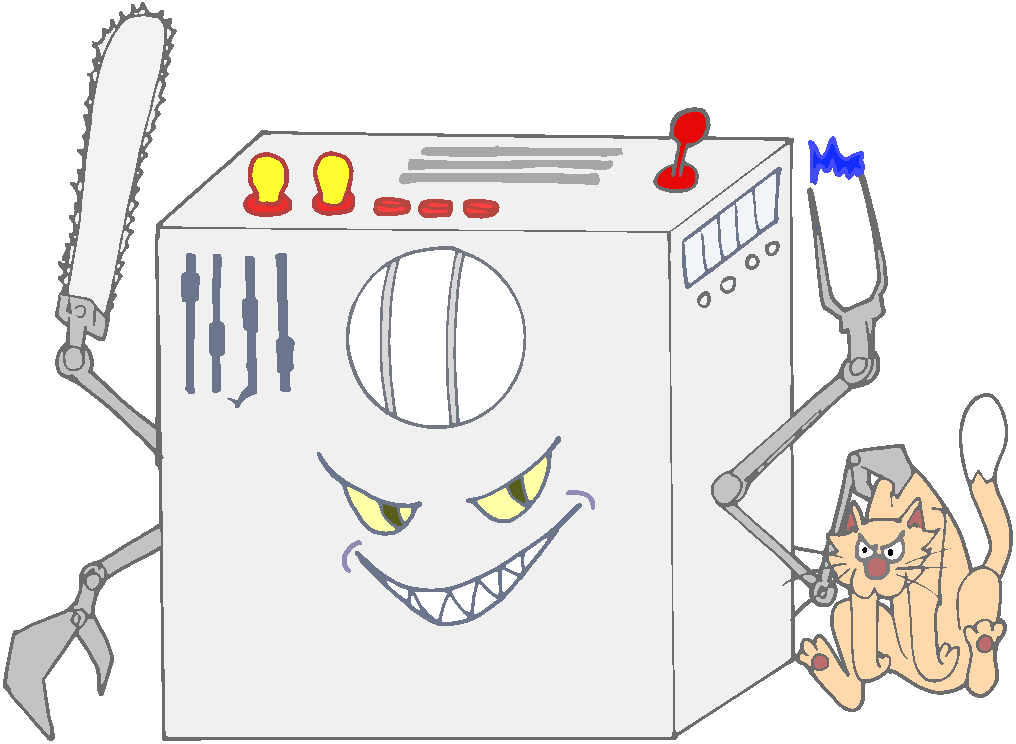
\includegraphics[height=2.5cm]{qc-color}};
    
    \node(E0) at (-6,0) {
\includegraphics[height=1cm]{ec-happy}};

    \uncover<2->{
      \node(EA) at (0,3) {
\includegraphics[height=1cm]{ec-happy}};
      \node(EB) at (0,-3) {
\includegraphics[height=1cm]{ec-happy}};
      \draw[->,decorate,decoration=snake] (E0) to (EA);
      \draw[->,decorate,decoration=snake] (E0) to (EB);
      \node[right=0.3cm of EA] {\bl{Public curve}};
      \node[right=0.3cm of EB] {\bl{Public curve}};
    }
    \uncover<3>{
      \node(ES) at (6,0) {
\includegraphics[height=1cm]{ec-happy}};
      \draw[->,decorate,decoration=snake] (EA) to (ES);
      \draw[->,decorate,decoration=snake] (EB) to (ES);
      \node[below=1em of ES] {\rd{Shared secret}};
    }
  \end{tikzpicture}
\end{frame}

%%

\begin{frame}{Hard Homogeneous Spaces\footcite{Couv}}
  \begin{block}{Principal Homogeneous Space}
    \emph{$\G\circlearrowright\E$}: A (finite) set $\E$ \emph{acted
      upon} by a group $\G$ \emph{faithfully} and \emph{transitively}:
    \begin{align*}
      * : \G × \E &→ \E\\
      \g * E &↦ E'
    \end{align*}
    \par\begin{description}
    \item[Compatibility:] \emph{$\g' * (\g * E) = (\g'\g)*E$} for all
      $\g,\g'\in\G$ and $E\in\E$;
    \item[Identity:] \emph{$\mathfrak{e} * E = E$} if and only if
      $\mathfrak{e}\in\G$ is the identity element;
    \item[Transitivity:] for all $E,E'\in\E$ there exist a
      \emph{unique $\g\in\G$} such that \emph{$\g*E'=E$}.
      \setlength{\itemsep}{2em}
    \item[Example:] the set of \emph{elliptic curves with complex
        multiplication} by $\O$\\
      is a PHS for the \emph{class group} $\Cl(\O)$.
    \end{description}
  \end{block}
\end{frame}

%%

\begin{frame}{Hard Homogeneous Spaces}
  \begin{block}{Hard Homogeneous Space (HHS)}
    A Principal Homogeneous Space \emph{$\G\circlearrowright\E$} such
    that:
    \begin{itemize}
    \item \emph{Evaluating} $E' = \g*E$ is \emph{easy};
    \item \emph{Inverting} the action is \emph{hard}.
    \end{itemize}
  \end{block}

  Discrete logarithms in $\G=〈\g〉$ are easy $\quad⇔\quad$ there is
  an effective isomorphism
  \begin{align*}
    \Z/N\Z &\longleftrightarrow \G\\
    a &↦ \g^a
  \end{align*}
  Then we like to see $\E$ as an \emph{HHS for $\Z/N\Z$}:
  \begin{align*}
    \Z/N\Z × \E &→ \E\\
    [a]E &↦ \g^a*E
  \end{align*}

  \centering
  \textbf{Warning:}~~~~~~\emph{$[a][b]E = [a+b]E$}~~~~~~!!!
\end{frame}

%%

\begin{frame}{HHS Diffie--Hellman}
  \begin{description}
  \item[Goal:] Alice and Bob have never met before. They are chatting
    over a public channel, and want to agree on a \emph{shared secret}
    to start a private conversation.
  \item[Setup:] They agree on a (large) \emph{HHS
      $\langle g\rangle\circlearrowright \E$} of order $N$.
  \end{description}

  \begin{center}
    \begin{tikzpicture}
      \node at (0,0) {\bf Alice};
      \node at (7,0) {\bf Bob};
      \node at (0,-1) {pick random \alert{$a\in\Z/N\Z$}};
      \node at (0,-1.5) {compute $E_A=[a]E_0$};
      \node at (7,-1) {pick random \alert{$b\in\Z/N\Z$}};
      \node at (7,-1.5) {compute $E_B=[b]E_0$};
      \draw[->]
      (1,-2) to node[auto] {$E_A$} (6,-2);
      \draw[->] (6,-2.5) to node[auto] {$E_B$} (1,-2.5);
      \node at (3.5,-3.5) {\emph{Shared secret} is \alert{$[a]E_B=[a+b]E_0=[b]E_A$}};
    \end{tikzpicture}
  \end{center}  
\end{frame}

%%

\begin{frame}{HHSDH from complex multiplication}
  \begin{columns}
    \begin{column}{0.6\textwidth}
      \textbf{Obstacles:}
      \begin{itemize}
      \item \emph{We don't want to wait for a quantum computer} for
        solving discrete logs in $\Cl(\O)$!
      \item Until then, even the \emph{group size} of $\Cl(\O)$ is
        \emph{unknown}.
      \item Only ideals of small norm (\emph{isogenies of small degree})
        are efficient to evaluate.
      \end{itemize}

      \textbf{Solution:}
      \begin{itemize}
      \item Restrict to elements of $\Cl(\O)$ of the form
        \[\g = \prod \a_i^{e_i}\]
        for a basis of $\a_i$ of \emph{small norm}.
      \item Equivalent to doing \emph{isogeny walks} of \emph{smooth
          degree}.
      \end{itemize}
    \end{column}
    \begin{column}{0.4\textwidth}
      \centering
      \begin{tikzpicture}
        \begin{scope}
          \def\crater{12}
          \def\jumpa{-8}
          \def\jumpb{9}
          \def\diam{2cm}

          \foreach \i in {1,...,\crater} {
            \draw[blue] (360/\crater*\i : \diam) to[bend right] (360/\crater*\i+360/\crater : \diam);
            \draw[red] (360/\crater*\i : \diam) to[bend right] (360/\crater*\i+\jumpa*360/\crater : \diam);
            \draw[green] (360/\crater*\i : \diam) to[bend right=50] (360/\crater*\i+\jumpb*360/\crater : \diam);
          }
          \foreach \i in {1,...,\crater} {
            \draw[fill] (360/\crater*\i: \diam) circle (2pt) +(360/\crater*\i: 0.4) node{$E_{\i}$};
          }
        \end{scope}
      \end{tikzpicture}
    \end{column}
  \end{columns}
\end{frame}

%% 

\begin{frame}
  \frametitle{CSIDH key exchange}

  \begin{columns}
    \begin{column}{0.55\textwidth}
      \begin{tikzpicture}
        \begin{scope}
          \def\crater{12}
          \def\jumpa{-8}
          \def\jumpb{9}
          \def\diam{2.5cm}
          
          \foreach \i in {1,...,\crater} {
            \pgfmathparse{int(mod(2^\i,13))}
            \let\exp\pgfmathresult
            \draw[fill] (360/\crater*\i: \diam) circle (2pt);
          }
          \uncover<2,6->{
            % Alice 1
            \myedge{0}{1}{blue}\myedge{1}{5}{red}\myedge{5}{6}{blue}\myedge{6}{3}{green}
          }
          \uncover<3,5>{
            % Bob 1
            \begin{scope}[dashed,thick]
              \myedge{0}{4}{red}\myedge{4}{8}{red}\myedge{8}{5}{green}\myedge{5}{6}{blue}
            \end{scope}
          }
          \uncover<5>{
            % Alice 2
            \myedge{6}{7}{blue}\myedge{7}{11}{red}\myedge{11}{0}{blue}\myedge{0}{9}{green}
          }
          \uncover<6->{
            % Bob 2
            \begin{scope}[dashed,thick]
              \myedge{3}{7}{red}\myedge{7}{11}{red}\myedge{11}{8}{green}\myedge{8}{9}{blue}
            \end{scope}
          }

          \draw (0 : \diam + 0.4cm) node {$E_0$};
          \uncover<2->{\draw (360/\crater*3 : \diam + 0.4cm) node {$E_A$};}
          \uncover<3->{\draw (360/\crater*6 : \diam + 0.4cm) node {$E_B$};}
          \uncover<5->{\draw (360/\crater*9 : \diam + 0.4cm) node {$E_{BA}\uncover<6->{=E_{AB}}$};}
        \end{scope}
      \end{tikzpicture}  
    \end{column}    
    \begin{column}{0.45\textwidth}
      \textbf{Public parameters:}
      \begin{itemize}
      \item A supersingular curve $E_0/\F_p$;
      \item A set of small prime degree isogenies.
      \end{itemize}
      \begin{enumerate}
      \item<2-> \textbf{Alice} takes a \alert{secret} random walk
        \emph{$ϕ_A:E_0\to E_A$} of length \emph{$O(\log p)$};
      \item<3-> \textbf{Bob} does the same;
      \item<4-> They publish \emph{$E_A$} and \emph{$E_B$};
      \item<5-> \textbf{Alice} repeats her secret walk \emph{$ϕ_A$}
        starting from \emph{$E_B$}.
      \item<6-> \textbf{Bob} repeats his secret walk \emph{$ϕ_B$}
        starting from \emph{$E_A$}.
      \end{enumerate}
    \end{column}
  \end{columns}
\end{frame}

%%

\begin{frame}{CSIDH data flow}
  \textbf{Your secret:} a vector of number of \emph{isogeny steps} for each degree
  \begin{center}
    \begin{tikzpicture}
      \node at (0,0) {
        $\bigl( \bl{5}, \rd{1}, \gr{-4}, \dots \bigr)$
      };
      \begin{scope}[xshift=3cm,xscale=0.3,yscale=0.2]
        \draw (0,0) -- (18,0);
        \draw[dotted] (0,5) -- (18,5) (0,-5) -- (18,-5);

        \foreach \i in {0,...,18} {
          \pgfmathparse{round(5*sin(125*\i))}
          \let\r\pgfmathresult
          \draw[very thick] (\i,0) -- (\i,\r);
        }
      \end{scope}
    \end{tikzpicture}
  \end{center}
  
  \bigskip
  
  \textbf{Your public key:} (the $j$-invariant of) a supersingular elliptic curve
  \begin{align*}
    j =\;\; &\mathtt{0x23baf75419531a44f3b97cc9d8291a275047fcdae0c9a0c0ebb993964f821f2}\\
            &\mathtt{0c11058a4200ff38c4a85e208345300033b0d3119ff4a7c1be0acd62a622002a9}
  \end{align*}
\end{frame}

%%

\begin{frame}{Quantum security}

  \textbf{Fact:} Shor's algorithm \emph{does not apply} to Diffie-Hellman
  protocols from \emph{group actions}.

  \begin{block}{Subexponential attack\hfill\emph{$\exp(\sqrt{\log p\log\log p})$}}
    \begin{itemize}
    \item Reduction to the \emph{hidden shift problem} by evaluating
      the class group action in \emph{quantum
        supersposition}~\footcite{childs+jao+soukharev10} (subexpoential cost);
    \item Well known reduction from the hidden shift to the
      \emph{dihedral (non-abelian) hidden subgroup problem};
    \item Kuperberg's algorithm\footcite{Kup,regev04,Kuperberg2013}
      solves the dHSP with a subexponential number of class group
      evaluations.
    \item Recent
      work\footcite{cryptoeprint:2018:432,cryptoeprint:2018:537,biasse2018note,Jao-etal-kuperberg-2018,cryptoeprint:2018:1059}
      suggests that $2^{64}$-qbit security is achieved somewhere in
      $512 < \log p < 1024$.
    \end{itemize}
  \end{block}
\end{frame}

%%

\begin{frame}
  \frametitle{Key exchange with supersingular curves (2011)}
  
  \begin{description}
  \item[Good news:] there is no action of a commutative class group.
  \item[Bad news:] there is no action of a commutative class group.
  \item[Idea:] Let \bl{Alice} and \rd{Bob} walk in two
    \emph{different isogeny graphs} on the \emph{same vertex set}.
  \end{description}

  \begin{columns}
    \begin{column}{0.6\textwidth}
      \centering
      \begin{tikzpicture}[scale=1.4]
        \begin{scope}[every node/.style={fill,black,circle,inner sep=2pt}]
          \node at (0,0)  (1){};
          \node at (0,4) (20){};
          \node at (2,1)  (16z){};
          \node at (-2,1)  (81z){};
          \node at (-1,2) (77z){};
          \node at (1,2)  (20z){};
          \node at (-2,3)  (85z){};
          \node at (2,3)  (12z){};
        \end{scope}

        \begin{uncoverenv}<1,3>
          \begin{scope}[blue,every loop/.style={looseness=50}]
            \path (1) edge (20) edge (16z) edge (81z);
            \path (20) edge[loop left] (20) edge[loop right] (20);
            \path (16z) edge (81z) edge (77z);
            \path (81z) edge (20z);
            \path (77z) edge (20z) edge (85z);
            \path (20z) edge (12z);
            \path (12z) edge[bend right=10] (85z) edge[bend left=10] (85z);
          \end{scope}
        \end{uncoverenv}
        
        \begin{uncoverenv}<2->
          \begin{scope}[red]
            \path (1) edge (85z) edge (81z) edge (12z) edge (16z);
            \path (20) edge (85z) edge (77z) edge (20z) edge (12z);
            \path (81z) edge (85z) edge (77z) edge (16z);
            \path (85z) edge (12z);
            \path (12z) edge (16z);
            \path (16z) edge (20z);
            \path (20z) edge[bend right=10] (77z) edge[bend left=10] (77z);
          \end{scope}
        \end{uncoverenv}
      \end{tikzpicture}
    \end{column}
    \begin{column}{0.4\textwidth}
      \small
      \emph{Figure:} \bl{$2$}- and \rd{$3$}-isogeny graphs on $\F_{97^2}$.
    \end{column}
  \end{columns}
\end{frame}

%%

\begin{frame}
  \frametitle{Key exchange with supersingular curves (2011)}

  \begin{itemize}
  \item Fix small primes \bl{$\ell_A$}, \rd{$\ell_B$};
  \item \emph{No canonical labeling} of the \bl{$\ell_A$}- and
    \rd{$\ell_B$}-isogeny graphs; \emph{however\dots}
  \end{itemize}

  \begin{center}
    \bf
    Walk of length \bl{$e_A$}\\
    $=$\\
    Isogeny of degree \bl{$\ell_A^{e_A}$}\\
    $=$\\
    Kernel \bl{$\langle P\rangle\subset E[\ell_A^{e_A}]$}
  \end{center}
  
  \begin{center}
    \begin{tikzpicture}
      \begin{scope}
        \draw (0,1.2) node[anchor=east,blue] {$\ker\phi=〈P〉\subset E[\ell_A^{e_A}]$};
        \draw (0,0.4) node[anchor=east,red] {$\ker\psi=〈Q〉\subset E[\ell_B^{e_B}]$};
        \draw (0,-0.4) node[anchor=east,blue] {$\ker\phi' = 〈\rd{\psi}(P)〉$};
        \draw (0,-1.2) node[anchor=east,red] {$\ker\psi' = 〈\bl{\phi}(Q)〉$};
      \end{scope}
      \begin{scope}[xshift=4.5cm,coils/.style={-angle 90,decorate,decoration={coil,aspect=0,amplitude=1pt}}]
        \large
        \node[matrix of nodes, ampersand replacement=\&, column sep=3cm, row sep=1.5cm] (diagram) {
          |(E)| $E$ \& |(Es)| $E/〈\bl{P}〉$ \\
          |(Ep)| {$E/〈\rd{Q}〉$} \& |(Eps)| {$E/〈\bl{P},\rd{Q}〉$}\\
        };
        \path[->,blue] (E) edge[coils] node[auto] {$\phi$} (Es);
        \path[->,blue] (Ep) edge[coils] node[auto,swap] {$\phi'$} (Eps);
        \path[->,red] (E) edge[coils] node[auto,swap] {$\psi$} (Ep);
        \path[->,red] (Es) edge[coils] node[auto] {$\psi'$} (Eps);
      \end{scope}
    \end{tikzpicture}
  \end{center}
\end{frame}

%%

\begin{frame}
  \frametitle{Supersingular Isogeny
    Diffie-Hellman\footcite{jao+defeo2011,defeo+jao+plut12}}

  \vspace{-1cm}

  \begin{columns}
    \begin{column}{0.4\textwidth}
      \begin{block}{}
        \emph{Parameters:}
        \begin{itemize}
          \setlength{\itemsep}{1.5ex}
        \item Prime $p$ such that $p+1 = \bl{\ell_A^a}\rd{\ell_B^b}$;
        \item Supersingular curve \emph{$E\simeq (\Z/(p+1)\Z)^2$};
        \item \bl{$E[\ell_A^a] = \cyc{P_A,Q_A}$};
        \item \rd{$E[\ell_B^b] = \cyc{P_B,Q_B}$}.
        \end{itemize}

        \emph{Secret data:}
        \begin{itemize}
          \setlength{\itemsep}{1.5ex}
        \item \bl{$R_A = m_AP_A + n_AQ_A$},
        \item \rd{$R_B = m_BP_B + n_BQ_B$},
        \end{itemize}
      \end{block}
    \end{column}
    \begin{column}{0.58\textwidth}
      \begin{center}
        \begin{tikzpicture}[coils/.style={-angle 90,decorate,decoration={coil,aspect=0,amplitude=1pt}}]
          \large
          \node[matrix of nodes, ampersand replacement=\&, column sep=4mm, row sep=2cm] (diagram) {
            \& |(1)| $E$ \\
            |(a)| \parbox{1.5cm}{$E/\cyc{\bl{R_A}}$\\\uncover<2->{{\footnotesize $\bl{\phi(}\rd{P_B}\bl{)}\\\bl{\phi(}\rd{Q_B}\bl{)}$}}} \& \&
            |(b)| \parbox{1.5cm}{$E/\cyc{\rd{R_B}}$\\\uncover<2->{{\footnotesize $\rd{\psi(}\bl{P_A}\rd{)}\\\rd{\psi(}\bl{Q_A}\rd{)}$}}}\\
            \normalsize $\frac{E/\cyc{\bl{R_A}}}{\alert{\bl{\phi(}\rd{R_B}\bl{)}}} \simeq$ \&
            |(ab)|  $E/\cyc{\bl{R_A},\rd{R_B}}$ \&
            \normalsize $\simeq \frac{E/\cyc{\rd{R_B}}}{\alert{\rd{\psi(}\bl{R_A}\rd{)}}}$\\
          };
          \small
          \path[blue] (1) edge[coils] node[auto,swap](phia) {$\phi$} (a);
          \path[red] (1) edge[coils] node[auto](phib) {$\psi$} (b);
          \path[red] (a) edge[coils] node[auto,swap](psia){$\psi'$} (ab);
          \path[blue] (b) edge[coils] node[auto](psib){$\phi'$} (ab);
          \uncover<3>{\path[dashed,->] (phia) edge node[auto]{\footnotesize $\bl{\phi(}\rd{R_B}\bl{)}$} (psia);}
          \uncover<3>{\path[dashed,->] (phib) edge node[auto,swap]{\footnotesize $\rd{\psi(}\bl{R_A}\rd{)}$} (psib);}
        \end{tikzpicture}
      \end{center}  
    \end{column}
  \end{columns}
\end{frame}

%%

\begin{frame}{From 10 minutes to 10ms in 20 years}
  \begin{tikzpicture}[xscale=1.3,gray,every node/.style={anchor=south}]
    \draw[->] (0,0) -- (11,0);
    \uncover<1->{
      \node at (1,-0.5) {1996};
      \draw (1,-0.1) -- +(0,0.3) node[blue]{Couveignes' key exchange};
    }
    \uncover<2->{
      \node at (3,-0.5) {2006};
      \draw (3,-0.1) -- +(0,1.3) node[blue]{Rostovstev \& Stolbunov (> 5 min)};
    }
    \uncover<3->{
      \node at (4,-0.5) {2011};
      \draw (4,-0.1) -- +(0,2.3) node[red]{SIDH (500ms) \tiny(Jao and D.)};
    }
    \uncover<4->{
      \node at (5,-0.5) {2012};
      \draw (5,-0.1) -- +(0,3.3) node[red]{SIDH (50ms) \tiny(D., Jao, Plût)};
    }
    \uncover<5->{
      \node at (6,-0.5) {2016};
      \draw (6,-0.1) -- +(0,4.3) node[red]{SIDH (30ms) \tiny(Costello, Longa, Naherig)};
    }
    \uncover<6->{
      \node at (7,-0.5) {2017};
      \draw (7,-0.1) -- +(0,5.3) node[red]{SIKE (10ms) \tiny(NIST candidate)};
    }
    \uncover<7->{
      \node at (8,-0.5) {2018};
      \draw (8,-0.1) -- +(0,2.3) node[blue]{CSIDH (50ms)};
    }
    \uncover<8>{
      \node at (9,-0.5) {2019};
      \draw (9,-0.1) -- +(0,3.3) node[blue]{CSIDH (35ms) \tiny(Meyer, Reith)};
    }
  \end{tikzpicture}
\end{frame}

%%

\begin{frame}{CSIDH vs SIDH}
  \centering
  \vspace{-3mm}
  \begin{tabular}{l *{2}{| @{\hspace{1em}}c@{\hspace{1em}}} }
    & \textbf{CSIDH} & \textbf{SIDH}\\
    \hline
    Speed (on x64 arch., NIST 1) & $\sim$ 35ms & $\sim$ 6ms\\
    Public key size (NIST 1) & 64B & 346B\\
    Key compression & \\
    \enskip{}\rotatebox[origin=c]{180}{$\Lsh$} speed & & $\sim$ 11ms\\
    \enskip{}\rotatebox[origin=c]{180}{$\Lsh$} size & & 209B\\
    Submitted to NIST & no & yes\\
    TRL & 4 & 6\\
    \hline
    Best classical attack & $p^{1/4}$ & $p^{1/4}\;\;$ ($p^{3/8}$)\\
    Best quantum attack & $\tildO\left(3^{\sqrt{\log_3 p}}\right)$ & $p^{1/6}\;\;$ ($p^{3/8}$)\\
    Key size scales & quadratically & linearly\\
    CPA security & yes & yes\\
    CCA security & yes & Fujisaki-Okamoto\\
    Constant time & it's complicated & yes\\
    \hline
    Non-interactive key exchange & yes & no\\
    \alert<2->{Signatures} & short but (slow $\mid$ do not scale) & big and slow
  \end{tabular}
\end{frame}

%%

\begin{frame}{Why prove a secret isogeny?}
  \begin{description}
  \item[Public:] Curves \emph{$E, E'$}
  \item[Secret:] An isogeny walk \emph{$E\to E'$}
  \end{description}

  \begin{block}{Why?}
    \begin{itemize}
    \item For interactive identification;
    \item For signing messages;
    \item For validating public keys (esp. SIDH);
    \item More\dots
    \end{itemize}
  \end{block}

  \begin{block}{Some properties}
    \newcolumntype{C}{>{\centering\arraybackslash}X}
    \begin{tabularx}{\columnwidth}{l *{4}C}
      & \multicolumn{2}{c}{\small Zero knowledge}\\
      & \small Statistical & \small Computational & \small Quantum resistance & \small Succinctness\\
      \hline
      CSIDH & \checkmark & & \checkmark/{\footnotesize sort of} & \\
      SIDH & & \checkmark & \checkmark &\\
      Pairings & & & & \checkmark\\
    \end{tabularx}
  \end{block}
\end{frame}

%%

\begin{frame}{Security assumptions in Isogeny-based Cryptography}
  \begin{goodblock}{Isogeny walk problem}
    \begin{description}
    \item[Input] Two isogenous elliptic curves \emph{$E,E'$} over
      \emph{$\F_q$}.
    \item[Output] A path \emph{$E\to E'$} in an isogeny graph.
    \end{description}
  \end{goodblock}

  \begin{mehblock}{SIDH problem (1)}
    \begin{description}
    \item[Input]
      Elliptic curves \emph{$E,E'$} over \emph{$\F_q$},
      isogenous of degree \bl{$\ell_A^{e_A}$}.
    \item[Output] The unique path \emph{$E\to E'$} of length
      \bl{$e_A$} in the \bl{$\ell_A$}-isogeny graph.
    \end{description}    
  \end{mehblock}
  
  \begin{badblock}{SIDH problem (2)}
    \begin{description}
    \item[Input]
      \begin{itemize}
      \item Elliptic curves \emph{$E,E'$} over \emph{$\F_q$},
        isogenous of degree \bl{$\ell_A^{e_A}$};
      \item The action of the isogeny on $E[\rd{\ell_B^{e_B}}]$.
      \end{itemize}
    \item[Output] The unique path \emph{$E\to E'$} of length
      \bl{$e_A$} in the \bl{$\ell_A$}-isogeny graph.
    \end{description}    
  \end{badblock}
\end{frame}

%%

\begin{frame}{A $\Sigma$-protocol from Diffie--Hellman\footnote{Kids, do
      not try this at home! Use Schnorr!}}
  \begin{columns}
    \begin{column}{0.55\textwidth}
      \begin{itemize}
      \item<1-> A key pair \emph{$(s, g^s)$};
      \item<2-> Commit to a \emph{random element $g^r$};
      \item<3-> Challenge with bit \emph{$b\in\{0,1\}$};
      \item<4-> Respond with \emph{$c = \alert<6->{r - b\cdot s\mod\#G}$};
      \item<5-> Verify that \emph{$g^c(g^s)^b = g^r$}.
      \end{itemize}

      \begin{block}{Zero-knowledge}<6->
        \centering
        Does not leak because:\\
        \alert{$c$ is uniformly distributed} and independent from $s$.
      \end{block}

      \begin{uncoverenv}<7->
        Unlike Schnorr, compatible with\\
        \emph{group action Diffie--Hellman}.
      \end{uncoverenv}
    \end{column}  
    \begin{column}{0.40\textwidth}
      \centering
      \begin{tikzpicture}
        \node (g) at (0,0) {\alt<-6>{$g$}{$E_1$}};
        \node (gs) at (3,0) {\alt<-6>{$g^s$}{$E_s$}};
        \path[->] (g) edge node[auto]{\alt<-6>{$s$}{$g^s$}} (gs);
        \uncover<2->{
          \node (gr) at (1.5,-3) {\alt<-6>{$g^r$}{$E_r$}};
          \path[->] (g) edge node[auto,swap]{\alt<-6>{$r$}{$g^r$}} (gr);
        }
        \uncover<4->{
          \path[dashed,->] (gs) edge node[auto]{\alt<-6>{$r-s$}{$g^{r-s}$}} (gr);
        }
      \end{tikzpicture}
    \end{column}  
  \end{columns}
\end{frame}

%%

\begin{frame}{The trouble with groups of unknown structure}
  \begin{columns}
    \begin{column}{0.5\textwidth}
      In CSIDH secrets look like:
      $g^{\vec{s}} = \bl{g_2^{s_2}}\rd{g_3^{s_3}}\gr{g_5^{s_5}}\cdots$
      \begin{itemize}
      \item the elements $g_i$ are fixed,
      \item the secret is the exponent vector
        \emph{$\vec{s}=(s_2,s_3,\dots)\in[-B,B]^n$},
      \item secrets must be sampled in a box \emph{$[-B,B]^n$} ``large
        enough''\dots
      \end{itemize}

      \begin{block}{The leakage}<2->%
        With \emph{$\vec{s},\vec{r}\from[-B,B]^n$}, the distribution of
        \emph{$\vec{r}-\vec{s}$} \alert{depends on the long term secret $\vec{s}$!}
      \end{block}
    \end{column}
    \begin{column}{0.45\textwidth}
      \centering
      \begin{tikzpicture}[scale=0.3]
        \draw (-2,2) node{$+B$} (-2,-2) node{$-B$};
        \draw (0,0) -- (18,0);
        \draw[dotted] (0,2) -- (18,2) (0,-2) -- (18,-2);

        \draw (8,-4) node {\Large$-$};
        
        \draw (-2,-6) node{$+B$} (-2,-10) node{$-B$};
        \draw (0,-8) -- (18,-8);
        \draw[dotted] (0,-6) -- (18,-6) (0,-10) -- (18,-10);

        \uncover<2->{
          \draw (8,-12) node {\Large$=$};
        
          \draw (-2,-15) node{$+B$} (-2,-19) node{$-B$};
          \draw (0,-17) -- (18,-17);
          \draw[dotted] (0,-15) -- (18,-15) (0,-19) -- (18,-19);
        }
      
        \foreach \i in {0,...,18} {
          \pgfmathparse{round(2.2*sin(140*\i))}
          \let\s\pgfmathresult
          \pgfmathparse{round(2.2*cos(125*\i))}
          \let\r\pgfmathresult
          \draw[very thick] (\i,0) -- (\i,\r);
          \draw[very thick] (\i,-8) -- (\i,-8+\s);
          \uncover<2->{
            \draw[very thick] (\i,-17) -- (\i,-17+\r-\s);
          }
        }
      \end{tikzpicture}
    \end{column}
  \end{columns}
\end{frame}

%%

\begin{frame}{The two fixes}
  \begin{block}{Do like the lattice people}
    \emph{SeaSign}: D. and Galbraith 2019
    \begin{itemize}
    \item Use \emph{Fiat--Shamir with aborts} (Lyubashevsky 2009).
    \item[--] Huge increase in signature size and time.
    \item Compromise signature size/time with public key size (still
      slow).
    \end{itemize}
  \end{block}

  \begin{block}{Compute the group structure and stop whining}
    \emph{CSI-FiSh}: Beullens, Kleinjung and Vercauteren 2019
    \begin{itemize}
    \item Already suggested by Couveignes (1996) and Stolbunov (2006).
    \item Computationally intensive (\emph{subexponential parameter generation}).
    \item Decent parameters, e.g.: \emph{263 bytes, 390 ms, @NIST-1.} 
    \item[--] Technically not post-quantum (signing requires solving ApproxCVP).
   \end{itemize}
  \end{block}
\end{frame}

%%

\begin{frame}{Rejection sampling}
  \begin{columns}
    \begin{column}{0.5\textwidth}
      \begin{itemize}
      \item Sample \emph{long term secret $\vec{s}$} in the usual box \emph{$[-B,B]^n$},
      \item Sample \emph{ephemeral $\vec{r}$} in a larger box
        \emph{$[-(\delta+1)B,(\delta+1)B]^n$},
      \item Throw away \emph{$\vec{r}-\vec{s}$} if it is out of the box
        \emph{$[-\delta B,\delta B]^n$}.
      \end{itemize}

      \begin{block}{Zero-knowledge}
        \emph{Theorem:} $\vec{r}-\vec{s}$ is uniformly distributed in
        \emph{$[-\delta B,\delta B]^n$}.
      \end{block}

      \emph{Problem:} set $\delta$ so that rejection probability is
      low.
    \end{column}
    \begin{column}{0.5\textwidth}
      \centering
      \begin{tikzpicture}[scale=0.3]
        \draw (-3,3) node{$+(\delta+1)B$} (-3,-3) node{$-(\delta+1)B$};
        \draw (0,0) -- (18,0);
        \draw[dotted] (0,3) -- (18,3) (0,-3) -- (18,-3);

        \draw (8,-5) node {\Large$-$};
        
        \draw (-2,-7.5) node{$+B$} (-2,-8.5) node{$-B$};
        \draw (0,-8) -- (18,-8);
        \draw[dotted] (0,-7.5) -- (18,-7.5) (0,-8.5) -- (18,-8.5);

        \draw (8,-12) node {\Large$=$};
        
        \draw (-2,-14.5) node{$+\delta B$} (-2,-19.5) node{$-\delta B$};
        \draw (0,-17) -- (18,-17);
        \draw[dotted] (0,-14.5) -- (18,-14.5) (0,-19.5) -- (18,-19.5);
      
        \foreach \i in {0,...,18} {
          \pgfmathparse{round(60*random()-30)/10}
          \let\r\pgfmathresult
          \pgfmathparse{round(2*random()-1)/2}
          \let\s\pgfmathresult
          \draw[very thick] (\i,0) -- (\i,\r);
          \draw[very thick] (\i,-8) -- (\i,-8+\s);
          \draw[very thick] (\i,-17) -- (\i,-17+\r-\s);
        }
      \end{tikzpicture}
    \end{column}
  \end{columns}
\end{frame}

%%

\begin{frame}{SeaSign Performance (NIST-1)}
  \centering
  \begin{tabular}{l  c  c  c }
    & \bf $t=1$ bit challenges
    & \bf $t=16$ bits challenges
    & \bf PK compression \\
    \hline
    Sig size
    & \alert{20 KiB} & \gr{978 B} & 3136 B\\
    PK size
    & 64 B & \alert{4 MiB} & 32 B\\
    SK size
    & 32 B & 16 B & \alert{1 MiB} \\
    Est. keygen time
    & 30 ms & \alert{30 mins} & \alert{30 mins} \\
    Est. sign time
    & \alert{30 hours} & 6 mins & 6 mins \\
    Est. verify time
    & \alert{10 hours} & 2 mins & 2 mins \\
    \hline
    Asymptotic sig size
    & $O(\lambda^2\log(\lambda))$ & $O(\lambda t\log(\lambda))$ & $O(\lambda^2 t)$\\[2em]
    \multicolumn{4}{c}{\bf Speed/size compromises by Decru, Panny and Vercauteren 2019}\\
    \hline
    {Sig size}
    & 36 KiB & 2 KiB & ---\\
    {Est. sign time}
    & 30 mins & 80 s & ---\\
    {Est. verify time}
    & 20 mins & 20 s & ---
  \end{tabular}
\end{frame}

%%

\begin{frame}{CSI-FiSh~\footcite{beullens:2019}}
  \begin{itemize}
  \item Record breaking class group computation for CSIDH-512, hard to
    scale to larger primes;
  \item Effectively (but not asymptotically) makes CSIDH into an HHS:
    \begin{itemize}
    \item Compatible with secret sharing in the exponent, yields decent
      threshold signatures.\footcite{cryptoeprint:2019:1288}
    \end{itemize}
  \end{itemize}
  
  \centering
  \begin{tabular}{r r r | r r r | r r r }
    $S$ & $t$ & $k$ & $|\mathrm{sk}|$ & $|\mathrm{sk}|$ & $|\mathrm{sig}|$ & KeyGen & Sign & Verify \\
    \hline
    $2^1$    & $56$ & $16$ & 16 B & 128 B & 1880 B & 100 ms & 2.92 s & 2.92 s\\
    $2^2$    & $38$ & $14$ & 16 B & 256 B & 1286 B & 200 ms & 1.98 s & 1.97 s\\
    $2^3$    & $28$ & $16$ & 16 B & 512 B &  956 B & 400 ms & 1.48 s & 1.48 s\\
    $2^4$    & $23$ & $13$ & 16 B &  1 KB &  791 B & 810 ms & 1.20 s & 1.19 s\\
    $2^6$    & $16$ & $16$ & 16 B &  4 KB &  560 B & 3.3 s  & 862 ms & 859 ms\\
    $2^8$    & $13$ & $11$ & 16 B & 16 KB &  461 B & 13 s   & 671 ms & 670 ms\\
    $2^{10}$ & $11$ &  $7$ & 16 B & 64 KB &  395 B & 52 s   & 569 ms & 567 ms\\
    $2^{12}$ &  $9$ & $11$ & 16 B &256 KB &  329 B & 3.5 m  & 471 ms & 469 ms\\
    $2^{15}$ &  $7$ & $16$ & 16 B &  2 MB &  263 B & 28 m   & 395 ms & 393 ms
  \end{tabular}
\end{frame}

%%

\begin{frame}{A $Σ$-protocol for SIDH}
  \begin{columns}
    \begin{column}{0.6\textwidth}
      \begin{tikzpicture}
        \large
        \node[matrix of nodes, ampersand replacement=\&, column sep=3cm, row sep=1.3cm] (diagram) {
          |(E)| $E$ \& |(Es)| $E/〈\bl{S}〉$ \\
          |(Ep)| {\uncover<2->{$E/〈\rd{P}〉$}} \& |(Eps)| {\uncover<2->{$E/〈\rd{P,\bl{S}}〉$}}\\
        };
        \path[blue] (E) edge node[auto] {$\phi$} (Es);
        \uncover<2->{\path[blue] (Ep) edge node[auto,swap] {\alt<5>{$\phi'$}{\phantom{$\phi'$}?}} (Eps);}
        \uncover<2->{\path[red] (E) edge node[auto,swap] {\alt<3,6>{$\psi$}{?}} (Ep);}
        \uncover<2->{\path[red] (Eps) edge node[auto,swap] {\alt<4,6>{$\psi'$}{?}} (Es);}
      \end{tikzpicture}
    \end{column}
    \begin{column}{0.35\textwidth}
      \begin{mehblock}{$\frac{1}{3}$-soundness}
        Secret \bl{$\phi$} of degree \bl{$\ell_A^{e_A}$}.
      \end{mehblock}
    \end{column}
  \end{columns}

  \begin{enumerate}
  \item<2-> Choose a random point \rd{$P\in E[\ell_B^{e_B}]$}, compute the diagram;
  \item<2-> Publish the curves $E/〈\rd{P}〉$ and $E/〈\rd{P,\bl{S}}〉$;
  \item<3-> The verifier challenges to reveal \emph{one out of the 3}
    sides
    \begin{itemize}
    \item<3-> Isogenies \rd{$\psi,\psi'$} (degree \rd{$\ell_B^{e_B}$})
      unrelated to secret;
    \item<5-> Isogeny \bl{$\phi'$} conjectured to not reveal useful
      information on \bl{$\phi$}.
    \end{itemize}
  \end{enumerate}

  \begin{badblock}{Improving to $\frac{1}{2}$-soundness}<6->
    \begin{itemize}
    \item Reveal \rd{$\psi,\psi'$} simultaneously;
    \item Reveals action of \bl{$\phi$} on $E[\rd{\ell_B^{e_B}}]\quad⇒\quad$
      Stronger security assumption.
    \end{itemize}
  \end{badblock}
\end{frame}

%%

\begin{frame}{SIDH signature performance (NIST-1)}
  According to Yoo, Azarderakhsh, Jalali, Jao and Vladimir Soukharev
  2017:
  \begin{description}
  \item[Size:] $\approx 100 KB$,
  \item[Time:] seconds.
  \end{description}

  \pause
  
  \begin{goodblock}{Galbraith, Petit and Silva 2017}
    \begin{itemize}
    \item Concept similar to \emph{CSI-FiSh}: exploits \emph{known
        structure of endomorphism ring};
    \item Statistical zero knowledge (under heuristic assumptions);
    \item Based on the generic isogeny walk problem\\
      (requires \emph{special starting curve}, though);
    \item Size/performance comparable to Yoo \textit{et al.} (and possibly
      slower).
    \end{itemize}
  \end{goodblock}
\end{frame}

%%

\begin{frame}{Weil pairing and isogenies}
  \begin{block}{Theorem}
    Let \emph{$ϕ:E→E'$} be an isogeny and \emph{$\hat{ϕ}:E'→E$} its dual. \\
    Let \emph{$e_N$} be the Weil pairing of $E$ and \emph{$e_N'$} that
    of $E'$. %
    Then, for
    \[e_N(P,\hat{ϕ}(Q)) = e_N'(ϕ(P),Q),\]
    for any \emph{$P∈E[N]$} and \emph{$Q∈E'[N]$}.
  \end{block}
  
  \begin{block}{Corollary}
    \[e_N'(ϕ(P),ϕ(Q)) = e_N(P,Q)^{\deg ϕ}.\]
  \end{block}
\end{frame}

%%

\begin{frame}{Pairing proofs: what for?}
  \begin{itemize}
  \item<1-> Non-interactive, not post-quantum, not zero knowledge;
  \item<2-> Useful for (partially) validating SIDH public keys;
  \item<3-> \alert{Succinct:} proof size, verification time independent
    of walk length!
  \end{itemize}
\end{frame}

%%

{
  \setbeamercolor{background canvas}{bg=black}
  \begin{frame}[plain]
    \begin{tikzpicture}[remember picture,overlay]
      \node(pic)[at=(current page.center)] {
        \includegraphics[width=\paperwidth]{hodl.jpg}
      };
    \end{tikzpicture}
  \end{frame}
}

%%

\begin{frame}{Distributed lottery}
  Participants \textbf{A, B, \dots, Z} want to agree on a random
  winning ticket.

  \begin{block}{Flawed protocol}
    \begin{itemize}
    \item Each participant \emph{$x$} broadcasts a random string
      \emph{$s_x$};
    \item Winning ticket is \emph{$H(s_A, \dots, s_Z)$}.
    \end{itemize}
  \end{block}

  \pause

  \begin{block}{Fixes}
    \begin{itemize}
    \item Make the hash function \textbf{sloooooooooooooooooooooooooooow};
    \item<3> Make it possible to verify \emph{$w = H(s_A, \dots, s_Z)$} \textbf{fast}.
    \end{itemize}
  \end{block}
\end{frame}

%%

\begin{frame}{Verifiable Delay Functions (Boneh, Bonneau, Bünz, Fisch 2018)}
  \begin{block}{Wanted}
    Function (family) \emph{$f:X\to Y$} s.t.:

    \begin{itemize}
    \item Evaluating $f(x)$ takes \emph{long time}:
      \begin{itemize}
      \item \emph{uniformly} long time,
      \item on almost all random inputs $x$,
      \item even after having seen many values of $f(x')$,
      \item even given \emph{massive number of processors};
      \end{itemize}
    \item Verifying $y=f(x)$ is \emph{efficient}:
      \begin{itemize}
      \item ideally, exponential separation between evaluation and
        verification.
      \end{itemize}
    \end{itemize}
  \end{block}
\end{frame}

%%

\begin{frame}{Sequentiality}
  Ideal functionality:

  \[y = f(x) = \underbrace{H(H(\cdots(H(x))))}_{T \text{ times}}\]

  \begin{itemize}
  \item \emph{Sequential} assuming hash output ``unpredictability'',
  \item but how do you verify?
  \end{itemize}
\end{frame}

%%

\begin{frame}{Isogeny VDF ($\mathbb{F}_p$-version)}
  \begin{block}{(Trusted) Setup}
    \begin{itemize}
    \item Pairing friendly \emph{supersingular} curve $E/\mathbb{F}_p$\\
      \emph{with unknown endomorphism ring}
    \item Isogeny \emph{$\phi:E\to E'$} of degree \emph{$2^T$},
    \item Point \emph{$P\in E[(N,\pi-1)]$}, image \emph{$\phi(P)$}.
    \end{itemize}
  \end{block}

  \begin{block}{Evaluation}
    \begin{description}
    \item[Input:] random \emph{$Q\in E'[(N,\pi+1)]$},
    \item[Output:] \emph{$\hat\phi(Q)$}.
    \end{description}
  \end{block}

  \begin{block}{Verification}
    \large
    \[e_N(P,\hat\phi(Q)) \quad\overset{?}{=}\quad e_N(\phi(P),Q).\]
  \end{block}
\end{frame}

%%

\begin{frame}{Conclusion}
  \begin{itemize}
  \item Repeat with me: \emph{I need isogeny-based crypto!}
  \item \emph{Different} isogeny graphs enable different applications,
    different \emph{security assumptions}.
  \item Public key encryption based on isogenies \emph{is a reality},
    although maybe not your \#1 choice for TLS.
  \item Post-quantum isogeny signatures are still \emph{far from
      practical}.
  \item \emph{Practical} isogeny signatures do exists (CSI-FiSh); you
    can start using them now if you are an isogeny hippie, are ok
    for threshold signatures, but they \emph{do not scale}.
  \item Pairing-based isogeny proofs are usable, but not interesting
    for signatures: look into \emph{succinctness}, instead!
  \end{itemize}
\end{frame}

%% 

\begin{frame}[plain]
  \centering
  \begin{tikzpicture}[remember picture,overlay]
    \begin{scope}[xscale=1.7,yshift=-15,opacity=0.8]
      \def\crater{12}
      \def\jumpa{-8}
      \def\jumpb{9}
      \def\diam{5cm}

      \foreach \i in {1,...,\crater} {
        \draw[blue] (360/\crater*\i : \diam) to[bend right] (360/\crater*\i+360/\crater : \diam);
        \draw[red] (360/\crater*\i : \diam) to[bend right] (360/\crater*\i+\jumpa*360/\crater : \diam);
        \draw[green] (360/\crater*\i : \diam) to[bend right=50] (360/\crater*\i+\jumpb*360/\crater : \diam);
      }
    \end{scope}
    
    \draw (0,0.5) node{\Huge\bf Thank you};
    \draw (0,-1.1) node{\large\url{https://defeo.lu/}};
    \draw (0,-1.8) node{\large
\includegraphics[height=0.9em]{twitter.png}~\href{https://twitter.com/luca_defeo}{@luca\_defeo}};
  \end{tikzpicture}
\end{frame}

%%

\begin{frame}[allowframebreaks]
  \frametitle{Article citations}

  \defbibfilter{books}{\type{book} \or \type{booklet} \or \type{thesis}
    \or \type{report} \or \type{collection} \or \type{manual}
    \or \type{periodical} \or \type{proceedings}}
  \defbibfilter{articles}{\not \(\type{book} \or \type{booklet} \or \type{thesis}
    \or \type{report} \or \type{collection} \or \type{manual}
    \or \type{periodical} \or \type{proceedings}\)}

  \beamertemplatearticlebibitems
  \printbibliography[filter=articles]
\end{frame}

\end{document}


% LocalWords:  Isogeny abelian isogenies hyperelliptic supersingular Frobenius
% LocalWords:  isogenous


